\graphicspath{ {A1-MCD/Figures/} }

\section{Class and data structures}
\label{App:A1}

The linear optics package has been written in object-oriented Python
and is broken down in four principal modules:
\begin{itemize}
  \item \underline{\texttt{BeamLineElement}:} provides the various
    beam-line elements required to build a description of the beam
    line.
    Each individual element, such as a drift, quadrupole, etc., is
    described in a class derived from the \texttt{BeamLineElement}
    parent class.
  \item \underline{\texttt{BeamLine}:} provides code to assemble the
    elements into a coherent beam line.
    \texttt{BeamLine} is a singleton class to ensure that two beam
    lines can not be simulated in a single run of the package.
    The \texttt{extrapolateBeam} class is derived from
    the \texttt{Beam} class to handle the propagation of beam
    envelopes without the need to track individual particles.
  \item \underline{\texttt{Beam}:} provides code to calculate
    ensemble properties of the beam such as emittance.
    The ensemble properties are stored as instance attributes of
    the \texttt{Beam} class.
  \item \underline{\texttt{Particle}:} provides code to record beam
    particles at positions along the beam line.
    The module provides the singleton \texttt{ReferenceParticle}
    class derived from the \texttt{Particle} class.
\end{itemize}
The relationships between the principal modules is illustrated in
figure~\ref{App:Fig:SASD}.
The single \texttt{BeamLine} instance represents a beam line made up
of many \texttt{BeamLineElements} (indicated by the double-headed
arrow).
In turn, many beams may be passed through the single \texttt{BeamLine}
instance.
\begin{figure}
  \begin{center}
    \includegraphics[width=0.95\textwidth]{sasd.pdf}
  \end{center}
  \caption{
    Schematc diagram of the relationships between the principal
    classes that make up the linear optics package.
    The double-headed arrows indicate a many-to-one relationship
    between the objects; the arrow head points to the object which
    has only one instance.
    The classes indicated in grey are derived from the class indicated
    in black over which they are plotted.
  }
  \label{App:Fig:SASD}
\end{figure}

Other modules: \texttt{BeamIO}, \texttt{LaTeX},
\texttt{PhysicalConstants}, \texttt{Report}, \texttt{Simulation},
\texttt{UserFramework}, and \texttt{Visualise}
support the principal modules or provide services.
The data structure is implemented as attributes of the instances of the 
various classes.
This section describes the implementation of the various modules, the
classes of which they are composed, and how access to the data is
provided.

Each class has methods by which to access a list of the class
instances and a Boolean flag by which to generate debug print out (see
table~\ref{Tab:ClassAttributeAccess}).
\begin{table}[h]
  \caption{Methods by which to set and access class attributes.}
  \label{Tab:ClassAttributeAccess}
  \begin{center}
    \begin{tabular}{|l|c|l|p{7cm}|}
      \hline
      \textbf{Method}          & \textbf{Argument} & \textbf{Return}            & \textbf{Comment}                      \\
      \hline
      \texttt{getinstances()}  &                   & List of instances of class & For singleton classes such as
                                                                                  \texttt{BeamLine}, \texttt{getinstances()}
                                                                                  returns a single instance rather than a list. \\
      \texttt{setDebug(Debug)} & Boolean           &                            & Sets flag to generate debug print-out \\
      \texttt{getDebug()}      &                   & Boolean debug flag         & If True, generate debug print-out     \\
      \texttt{setAll2None()}   &                   &                            & Set all instance attributes to
                                                                                  \texttt{None} at start of instantiation. \\
      \texttt{SummaryStr()}    &                   & String                     & Text sring to record parameters in debug
                                                                                  print out. \\
      \hline
    \end{tabular}
  \end{center}
\end{table}

\pagebreak

\subsection{\texttt{BeamLine}}

\texttt{BeamLine} is a singleton class that sets up the beam line
geometry and provides methods to track particles through the beam line
using the transfer matarices defined in section~\ref{SubSubSect:BLE}.
The beam-line geometry is provided in the form of a ``\texttt{csv}''
file read using \texttt{pandas}.
The format of the ``\texttt{csv}'' file is defined in
section~\ref{SubSubSect:??}.
Alternatively, if a data file written using the \texttt{BeamIO}
package is being read, the beam-line geometry is read from the top of
the data file.
The instance of the \texttt{BeamLine} class is created when the first
record of the data file is read.

\subsubsection{Instantiation} ~\newline
\noindent
The call to instantiate the \texttt{BeamLineElenent} class is:
\begin{center}
  \texttt{BeamLine(BeamLineSpecificationCSVfile, readDataFile)}
\end{center}
\texttt{BeamLineSpecificationCSVfile} is a the full path of the CSV
file containing the beam-line specificiation.
\texttt{readDataFile} is a boolean flag.
If \texttt{readDataFile} is set to \texttt{True}, then the \texttt{BeamLine}
instance will be created and the beam-line geometry will be read from
the header of the BeamIO data file.
If \texttt{readDataFile} is not set or is set to \texttt{False}, the
beam-line geometry will be read from \\
\noindent \texttt{BeamLineSpecificationCSVfile}.

\subsubsection{Instance attributes and access methods} ~\newline
\label{SubSubSect:BL:InstAttr}
\noindent
The instance attributes are presented in table~\ref{Tab:BL:Attributes}
and the access methods are summarised in table~\ref{Tab:BL:AccessMethods}.
\begin{table}[h]
  \caption{
    Definition of attributes of instances of
    the \texttt{BeamLine} class.
  }
  \label{Tab:BL:Attributes}
  \begin{center}
    \begin{tabular}{|l|c|p{8.5cm}|}
      \hline
      \textbf{Attribute} & \textbf{Type} & \textbf{Comment}                                                                  \\
      \hline
      \texttt{BeamLineSpecificationCSVfile}$^*$ & path      & Full path to beam-line specification \texttt{csv} file.        \\
      \texttt{BeamLineParamPandasInstance}      & dataframe & Pandas data frame containing beam-line specification.          \\
      \texttt{Element}                          & list      & List of instances of \texttt{BeamLineElement} class containing
                                                              pointers to the elements that make up the beam line.           \\
      \hline
    \end{tabular}
  \end{center}
\end{table}
\begin{sidewaystable}[h]
  \caption{
    Definition of access methods for the \texttt{BeamLine}
    class. 
  }
  \label{Tab:BL:AccessMethods}
  \begin{center}
    \begin{tabular}{|c|c|p{10cm}|}
      \hline
      \textbf{Set method} & \textbf{Get method}  & \textbf{Comment}                                                              \\
      \hline
      \texttt{setSrcTrcSpc(SrcTrcSpc)} & \texttt{getSrcTrcSpc()} & Set trace space at source; SrcTrcSpc presented as \texttt{(1,6)}
                                                                   \texttt{np.ndarray}.                                          \\
                                         & \texttt{getinsance()} & Get instance of \texttt{BeamLine} class.                        \\
                       & \texttt{BeamLineSpecificationCSVfile()} & Get beam line specification csv file.                           \\
                             & \texttt{(getBeamLineParamPandas)} & Get pandas dat from containing beam-line specification.         \\
                                         & \texttt{getElement()} & get list of \texttt{BeamLineElement} instances.                 \\
      \hline
    \end{tabular}
  \end{center}
\end{sidewaystable}

\subsubsection{Processing methods} ~\newline
\noindent
Table~\ref{Tab:BL:ProcMethods} presents the processing methods provided
in the \texttt{BeamLine} class.
\begin{sidewaystable}[h]
  \caption{
    Processing methods provided by the \texttt{BeamLine}
    class. 
  }
  \label{Tab:BL:ProcMethods}
  \begin{center}
    \begin{tabular}{|l|c|c|p{10cm}|}
      \hline
      \textbf{Method} & \textbf{Argument(s)} & \textbf{Return} & \textbf{Comment}                                            \\
      \hline
      \texttt{addBeamLine()}   &  & \texttt{Success} & Loops through pandas data frame and manages parsing and instanciation
                                                       of the beam line elements defined in the specification \texttt{csv} file.
                                                       Returns \texttt{Success} (bool) which is \texttt{True} if the beamline
                                                       has been set up OK and is \texttt{False} otherwise.                     \\
      \texttt{addFacility()}   &  &  & Manages the extraction of the facility parameters from the pandas data frame and the
                                       creation of the single instance of \texttt{Facility(BeamLineElement)}.                  \\
      \texttt{addSource()}     &  &  & Manages the extraction of the source parameters from the pandas data frame and the
                                       creation of the single instance of \texttt{Source(BeamLineElement)}.                  \\
      \texttt{parseFacility()} &  & \texttt{Name}, \texttt{K0}, \texttt{VCMVr} & Parses pandas data frane to extract
                                                                                 facility parameters.
                                                                                 Returns the facility \texttt{Name} (str), the
                                                                                 kinetic energy of the reference particle,
                                                                                 \texttt{K0} (float) in MeV, and the vacuum
                                                                                 chamber mother volume radius, \texttt{VCMVr}
                                                                                 (float) in m.                                 \\
      \texttt{parseSource()}   &  & \texttt{Name}, \texttt{Mode}, \texttt{Param} & Parses pandas data frane to extract
                                                                                 source parameters.
                                                                                 Returns \texttt{Name} (str), \texttt{Mode} (int)
                                                                                 \texttt{Param} (list) containing the parameters
                                                                                 required to instanciate source \texttt{Mode}. \\
      \texttt{addBeamLineElement(iBLE)} &  &  & Adds \texttt{BeamLineElement} instance \texttt{iBLE} to the list of instances of
                                                     \texttt{BeamLineElement} that make up the beam line.                      \\
      \texttt{checkConsistency()} &  & \texttt{Consistent} & Checks the consistency of the beam line representation in memory
                                                             with that requested in the specification \texttt{csv} file.
                                                             Returns \texttt{Consistent} (bool) which is \texttt{True} if the
                                                             beamline is consistent is \texttt{False} otherwise.                     \\
      \texttt{trackBeamn(NEvts, particleFILE)} &  &  & Generates \texttt{NEvts} (int) particles and tracks them through the
                                                       beam line. \\
      \hline
    \end{tabular}
  \end{center}
\end{sidewaystable}

\subsubsection{I/o methods} ~\newline
\noindent
Table~\ref{Tab:BL:IoMethods} presents the i/o methods provided in
the \texttt{BeamLine} class.
\begin{table}[h]
  \caption{
    I/o methods provided by the \texttt{BeamLine}
    class. 
  }
  \label{Tab:BL:IoMethods}
  \begin{center}
    \begin{tabular}{|l|c|c|p{7cm}|}
      \hline
      \textbf{Method} & \textbf{Argument(s)} & \textbf{Return} & \textbf{Comment}                                            \\
      \hline
      \texttt{csv2pandas(csvFILE)} & Path & pandas dataframe & Read CSV file to create pandas data frame.
                                                               \texttt{csvFILE} (path) is the full path to the \texttt{csv}   \\
      \texttt{pandasBeamLine()}    &      & pandas dataframe & Create pandas dataframe from \texttt{BeamLine} instance.       \\
      \texttt{getHeader()}         &      & List             & Prepares list of header fields for \texttt{pandasBeamLine}.    \\
      \texttt{readBeamLine(file)}  & Path & Boolean          & Called from \texttt{BeamIO}.  Reads \texttt{BeamLine} from data file. \\
      \hline
    \end{tabular}
  \end{center}
\end{table}

\subsubsection{Utilities} ~\newline
\noindent
Table~\ref{Tab:BL:UtilMethods} presents the utilities provided in
the \texttt{BeamLine} class.
\begin{table}[h]
  \caption{
    Utilities provided by the \texttt{BeamLine}
    class. 
  }
  \label{Tab:BL:UtilMethods}
  \begin{center}
    \begin{tabular}{|l|c|c|p{7cm}|}
      \hline
      \textbf{Method} & \textbf{Argument(s)} & \textbf{Return} & \textbf{Comment}                                            \\
      \hline
      \texttt{cleaninstance()} &      &          & Remove \texttt{BeamLine} instance.    \\
      \texttt{fixsz()}         &      & List     & Loop through \texttt{BeamLineElement} instances to
                                                   set $s$ and $z$ at exit.               \\
      \hline
    \end{tabular}
  \end{center}
\end{table}

\FloatBarrier

\pagebreak

\subsection{\texttt{Particle} and \texttt{ReferenceParticle}}
\label{SubSect:BLE:ParticleReferenceParticle}

The \texttt{Particle} class provides methods to transport particles
through the beam line.
The trace and phase space is recorded at the start and end of each
element.
The \texttt{ReferenceParticle} derived class is a singleton and
records the trajectory of the reference particle.

\subsubsection{\texttt{Particle}} ~\newline
\label{SubSubSect:BLE:Particle}

\paragraph{Instantiation}  ~\newline
\noindent
The call to instantiate the \texttt{Particle} class is:
\begin{center}
  \texttt{Particle(Species)}
\end{center}
\texttt{Species}, the type of particle to be propagated, is a string
containing the particle name.
At present valid particle \texttt{species} are
\texttt{proton}, \texttt{pion}, and \texttt{muon}.

\paragraph{Instance attributes and access methods} ~\newline
\label{Para:BLE:InstAttr}
\noindent
The instance attributes are presented in table~\ref{Tab:P:Attributes}
and the access methods are summarised in table~\ref{Tab:P:AccessMethods}.
\begin{table}[h]
  \caption{
    Definition of attributes of instances of the \texttt{Particle} class.
  }
  \label{Tab:P:Attributes}
  \begin{center}
    \begin{tabular}{|l|c|p{12cm}|}
      \hline
      \textbf{Attribute} & \textbf{Type} & \textbf{Comment}                                                                  \\
      \hline
      \texttt{Species}       & str   & Particle species; proton, muon or pion.                                                     \\
      \texttt{Location}      & list  & List of strings containing the unique \texttt{Name} of the \texttt{BeamLineElement} at
                                       the particle position is reported.                                                          \\
      \texttt{s}             & list  & List of floats recording $s$ coordinate at which particle position is reported.             \\
      \texttt{TraceSpace}    & list  & List of \texttt{np.ndarray} containing 6D trace space of particle at \texttt{s}.            \\
      \texttt{PhaseSpace}    & list  & List of \texttt{np.ndarray} containing 6D phase space (RPLC) of particle at \texttt{s}.     \\
      \texttt{LabPhaseSpace} & list  & List of \texttt{np.ndarray} containing 6D phase space (Lab) of particle at \texttt{s}.      \\
      \hline
    \end{tabular}
  \end{center}
\end{table}
\begin{sidewaystable}[h]
  \caption{
    Definition of access methods for the \texttt{Particle}
    class. 
  }
  \label{Tab:P:AccessMethods}
  \begin{center}
    \begin{tabular}{|c|c|p{9cm}|}
      \hline
      \textbf{Set method} & \textbf{Get method}  & \textbf{Comment}                                                      \\
      \hline
      \texttt{setSpecies}        & \texttt{getSpecies}        & Set/get particle species.                                \\
      \texttt{setLocation}       & \texttt{getLocation}       & Set/get list of locations location.                      \\
      \texttt{sets}              & \texttt{gets}              & Set/get list of $s$ coordinates.                         \\
      \texttt{setTraceSpace}     & \texttt{getTraceSpace}     & Set/get list of trace-space vectors.                     \\
      \texttt{setRPLCPhaseSpace} & \texttt{setRPLCPhaseSpace} & Set/get list of phase-space vectirs in RPLC coordinates. \\
      \texttt{setLabPhaseSpace}  & \texttt{getLabPhaseSpace}  & Set/get list of phase-space vectirs in Lab coordinates.  \\
      \texttt{resetParticleInstances} &                       & Resets list of particle instances preserving reference
                                                                particle as firt instance in the list.                   \\
      \texttt{recordParticle(Loc,z,s,TrcSpc)} &            & Records particle attributes.  Arguments: \texttt{Loc}$=$Location,
                                                                \texttt{z}$=z$, \texttt{s}$=s$, and
                                                                \texttt{TrcSpc}$=$trace space.                           \\
      \texttt{setSourceTraceSpace(TrcSpc)} &               & Sets \texttt{TrcSpc}$=$trace space at source.               \\
      \hline
    \end{tabular}
  \end{center}
\end{sidewaystable}

\paragraph{Processing methods} ~\newline % Here!
\noindent
Table~\ref{Tab:P:ProcMethods} presents the processing methods provided
in the \texttt{Particle} class.
\begin{sidewaystable}[h]
  \caption{
    Processing methods provided by the \texttt{Particle}
    class. 
  }
  \label{Tab:P:ProcMethods}
  \begin{center}
    \begin{tabular}{|l|c|c|p{10cm}|}
      \hline
      \textbf{Method} & \textbf{Argument(s)} & \textbf{Return} & \textbf{Comment}                                            \\
      \hline
      \texttt{fillPhaseSpaceAll()} & & Boolean & Fill phase space for all \texttt{Particle} instances.  Class Method.
                                                 Return \texttt{True} if successful.                                         \\
      \texttt{fillPhaseSpace()}    & & Boolean & Fill phase space for current \texttt{Particle} instance.
                                                 Return \texttt{True} if successful.                                         \\
      \texttt{initialiseSums()} &  &  & Initialises sums used to calculate covariance matrix.                                \\
      \texttt{incrementSums(iPrtcl)}  & \texttt{Particle} instance &  & Increment sums used to calculate covariance matrix.  \\
      \texttt{calcCovarianceMatrix()} &  &  & Calculate covariance matrix.                                                   \\
      \texttt{evaluateBeam()} &  &  & Work through locations and calculate parameters from covariance matrix.                 \\
      \texttt{calcRPLCPhaseSpace(nLoc)}& Int & np.ndarray & Calculate and return phase space in RPLCs at location \texttt{nLoc}. \\
      \texttt{RPLCTraceSpace2PhaseSpace(TrcSpc)} & np.ndarray & np.ndarray & Transform trace space to phase space in RPLCs.  \\
      \texttt{RPLCPhaseSpace2TraceSpace(TrcSpc)} & np.ndarray & np.ndarray & Transform phase space to trace space in RPLCs.  \\
      
      \hline
    \end{tabular}
  \end{center}
\end{sidewaystable}

\paragraph{I/o methods} ~\newline
\noindent
The i/o methods provided by the \texttt{Particle} class are listed in
table~\ref{Tab:P:IoMethods}.
\begin{sidewaystable}[h]
  \caption{
    I/o methods provided by the \texttt{Particle} class. 
  }
  \label{Tab:P:IoMethods}
  \begin{center}
    \begin{tabular}{|l|c|c|p{10cm}|}
      \hline
      \textbf{Method} & \textbf{Argument(s)} & \textbf{Return} & \textbf{Comment}                                          \\
      \hline
      \texttt{createParticleFile(path, file)} & Path, Str & Path    & Class method, kept for backward compatibility.          \\
      \texttt{flushNcloseParticleFile(file)}  & Path      &         & Class method, kept for backward compatibility.          \\
      \texttt{openParticleFile(path, file)}   & Path, Str &         & Class method, kept for backward compatibility.          \\
      \texttt{closeParticleFile(path, file)}  & Path, Str &         & Class method, kept for backward compatibility.          \\
      \texttt{readParticle(file)}             & Path      & Boolean & Read particle from input stream.  Called from \texttt{BeamIO}.
                                                                   \texttt{file} is full path to file. Return \texttt{True} if end
                                                                   of file.                                                   \\
      \texttt{writeParticle(file, clean)} & Path, boolean &      & Write particle to output stream.  
                                                                   \texttt{file} is full path to file. If \texttt{clean}, then
                                                                   clean particle instance after write.                    \\
      \texttt{writeParticleBDSIM(file, iLoc, clean)} & Path, integer, boolean &  & Write particle to BDSIM ascii file.
                                                                   \texttt{file} is full path to file.
                                                                   \texttt{iLoc} is the location along the beamm line at which
                                                                   to write the particle coordinates.
                                                                   If \texttt{clean}, then clean particle instance after write. \\
      \hline
    \end{tabular}
  \end{center}
\end{sidewaystable}


\paragraph{Utilities} ~\newline
\noindent
The utilities provided by the \texttt{Particle} class are listed in
table~\ref{Tab:P:UtilMethods}.
\begin{sidewaystable}[h]
  \caption{
    Utilities provided by the \texttt{Particle}
    class. 
  }
  \label{Tab:P:UtilMethods}
  \begin{center}
    \begin{tabular}{|l|c|c|p{10cm}|}
      \hline
      \textbf{Method} & \textbf{Argument(s)} & \textbf{Return} & \textbf{Comment}                                          \\
      \hline
      \texttt{cleanAllParticles()}&  &  & Delete all \texttt{Particle} instances including \texttt{ReferenceParticle}.     \\
      \texttt{cleanParticles()}   &  &  & Delete all \texttt{Particle} instances except \texttt{ReferenceParticle}.        \\
      \texttt{plotTraceSpaceProgression()} &  &  & Plot transverse trace space at each location.  Class method.  Writes file to
                                                   \texttt{99-Scratch/}.                                                   \\
      \texttt{plotLongitudinalTraceSpaceProgression()} &  &  & Plot longitudinal trace space at each location.  Class method.  Writes file to
                                                   \texttt{99-Scratch/}.                                                   \\
      \texttt{printProgression()} &  &  & Print particle parameters at each location.                      \\
      \texttt{getLines()}         &  &  & Returns lines to be used to create summary pandas data frame.                    \\
      \texttt{createReport()}     &  &  & Creates \texttt{csv} file containing summary of beam progression.                \\
      \hline
    \end{tabular}
  \end{center}
\end{sidewaystable}

\FloatBarrier

\subsubsection{\texttt{ReferenceParticle}} ~\newline
\label{SubSubSect:BLE:ReferenceParticle}

\paragraph{Instantiation}  ~\newline
\noindent
\texttt{ReferenceParticle} is a singleton derived class.
The call to instantiate the \texttt{ReferenceParticle} class is:
\begin{center}
  \texttt{ReferenceParticle(Species)}
\end{center}
\texttt{Species}, the type of particle to be propagated, is a string
containing the particle name.
At present valid particle \texttt{species} are
\texttt{proton}, \texttt{pion}, and \texttt{muon}.

\paragraph{Instance attributes and access methods} ~\newline
\label{Para:BLE:InstAttr}
\noindent
In addition to the instance attributes inheritted from the parent
class, the \texttt{ReferenceParticle} class provides the instance
attributes presented in table~\ref{Tab:RP:Attributes}
and the access methods are summarised in
table~\ref{Tab:RP:AccessMethods}.
\begin{table}[h]
  \caption{
    Definition of attributes of instances of the \texttt{ReferenceParticle} class.
  }
  \label{Tab:RP:Attributes}
  \begin{center}
    \begin{tabular}{|l|c|p{12cm}|}
      \hline
      \textbf{Attribute} & \textbf{Type} & \textbf{Comment}                                                                           \\
      \hline
      \texttt{\_sIn[]}   & list  & List of floats containing the $s$ coordinates at the entrance to the beam line elements along the
                                   locus of the reference particle trajectory.                                                        \\
      \texttt{\_sOut[]}  & list  & List of floats containing the $s$ coordinates at the exit to the beam line elements along the
                                   locus of the reference particle trajectory.                                                        \\
      \texttt{\_RrIn[]}  & list  & List of ndarrays containing the four-vector position in laboratory coordinates at the entrance to
                                   the beam line elements along the locus of the reference particle trajectory.                       \\
      \texttt{\_RrOut[]} & list  & List of ndarrays containing the four-vector position in laboratory coordinates at the exit to the
                                   beam line elements along the locus of the reference particle trajectory.                           \\
      \texttt{\_PrIn[]}  & list  & List of ndarrays containing the four-vector momentum in laboratory coordinates at the entrance to
                                   the beam line elements along the locus of the reference particle trajectory.                       \\
      \texttt{\_PrOut[]} & list  & List of ndarrays containing the four-vector momentum in laboratory coordinates at the exit to the
                                   beam line elements along the locus of the reference particle trajectory.                           \\
  \texttt{\_Rot2LabIn[]} & list  & List of ndarrays containing the rotation matrices taking RPLC to laboratory coordinates at the
                                   entrance to the beam line elements along the locus of the reference particle trajectory.           \\
 \texttt{\_Rot2LabOut[]} & list  & List of ndarrays containing the rotation matrices taking RPLC to laboratory coordinates at the
                                   exit to the beam line elements along the locus of the reference particle trajectory.               \\
      \hline
    \end{tabular}
  \end{center}
\end{table}
\begin{table}[h]
  \caption{
    Definition of access methods for the \texttt{ReferenceParticle}
    class. 
  }
  \label{Tab:RP:AccessMethods}
  \begin{center}
    \begin{tabular}{|c|c|p{7cm}|}
      \hline
      \textbf{Set method} & \textbf{Get method}  & \textbf{Comment}                                                      \\
      \hline
      \texttt{setRPDebug}        & \texttt{getRPDebug}        & Set/get \texttt{ReferenceParticle} debug flag.           \\
      \texttt{setsIn}            & \texttt{getsIn}            & Set/get \texttt{\_sIn}                                   \\
      \texttt{setsOut}           & \texttt{getsOut}           & Set/get \texttt{\_sOut}                                  \\
      \texttt{setRrIn}           & \texttt{getRrIn}           & Set/get \texttt{\_RrIn}                                  \\
      \texttt{setRrOut}          & \texttt{getRrOut}          & Set/get \texttt{\_RrOut}                                 \\
      \texttt{setPrIn}           & \texttt{getPrIn}           & Set/get \texttt{\_PrIn}                                  \\
      \texttt{setPrOut}          & \texttt{getPrOut}          & Set/get \texttt{\_PrOut}                                 \\
                                 & \texttt{getMomentumIn(iLoc)}  & Get magnitude of three-vector momentum at entrance of
                                                                   location \texttt{iLoc}                                \\
                                 & \texttt{getMomentumOut(iLoc)} & Get magnitude of three-vector momentum at exit of
                                   location \texttt{iLoc}                                                                \\
      \texttt{setRot2LabIn}      & \texttt{getRot2LabIn}      & Set/get \texttt{\_Rot2LabIn}                             \\
      \texttt{setRot2LabOut}     & \texttt{getRot2LabOut}     & Set/get \texttt{\_Rot2LabOut}                            \\
                                 & \texttt{getb0(iLoc)}       & Get $\beta_0$.                                           \\
                                 & \texttt{getg0b0(iLoc)}     & Get $\gamma_0 \beta_0$.                                  \\
      \texttt{setAllRP2None}     &                            & Set all \texttt{ReferenceParticle} attributes to None.   \\
      \hline
    \end{tabular}
  \end{center}
\end{table}
\begin{table}[h]
  \caption{
    Processing methods provided by the \texttt{ReferenceParticle}
    class. 
  }
  \label{Tab:RP:ProcMethods}
  \begin{center}
    \begin{tabular}{|l|c|c|p{4cm}|}
      \hline
      \textbf{Method} & \textbf{Argument(s)} & \textbf{Return} & \textbf{Comment}                                            \\
      \hline
      \texttt{setReferenceParticleAtSource()} &     & boolean & Set \texttt{ReferenceParticle} attributes at source.  Returns
                                                                True if success.                                             \\
      \texttt{setReferenceParticleAtDrift(iBLE)} & BLE & boolean & Set \texttt{ReferenceParticle} attributes at
                                                                   \texttt{BeamLineElement} (BLE) instance iBLE.  Returns
                                                                   True if success.                                          \\
      \hline
    \end{tabular}
  \end{center}
\end{table}

\FloatBarrier

\paragraph{Processing methods} ~\newline % Here!
\noindent
Table~\ref{Tab:RP:ProcMethods} presents the processing methods provided
in the \texttt{ReferenceParticle} class.

\paragraph{I/o methods} ~\newline
\noindent
The \texttt{ReferenceParticle} class provides no additional i/o methods.

\paragraph{Utilities} ~\newline
\noindent
The \texttt{ReferenceParticle} class provides no additional utilities.

\subsection{\texttt{Beam} and \texttt{extrapolateBeam}}
\label{SubSect:B}

The \texttt{Beam} class is in some sense a "sister" class to Particle.
Whereas an instance of \texttt{Particle} records the passage of a
particle travelling through the beam line, an instance
of \texttt{Beam} records the collective properties of the beam such as
emittance, as the beam progresses through the beam line.
The beam parameters reported in the attributes of an instance
of \texttt{Beam} are obtained by summing over \texttt{nEvtsMax}
particles to evaluate the covariance matrices by location.

The \texttt{extrapolatedBeam} class is derived from \texttt{Beam}.
An instance of \texttt{extrapolatedBeam} calculates the covariance
matrix at a location along the beam line and then uses the transfer
matrices to propagate the beam envelope.

\subsubsection{\texttt{Beam}}

\paragraph{Instantiation}\mbox{}\\
\noindent
The call to instantiate the \texttt{Beam} class is:
\begin{center}
  \texttt{Beam(InputDatafile, nEvtMax, outputCSVfile,
  startlocation, beamlineSpecificationCSVfile))}
\end{center}
\texttt{InputDatafile} is either the full path to a data file in one
of the formats specified in \texttt{BeamIO} or an instance of
the \texttt{BeamIO} class that refers to an existing data file that
can be read.
\texttt{nEvtMax} is the maximum number of events to read or process
using the \texttt{Beam} instance.
\texttt{outputCSVfile} is the full path to the output file, in CSV
format, contining the beam paramters at the locations traversed by the
beam. 
\texttt{startlocation} is the location along the beam line at which
propagation will start; if \texttt{startlocation} is absent or None
propagation will start at the source.
\texttt{beamlineSpecificationCSVfile} is the CSV file specifying the
beam line. \\
\texttt{beamlineSpecificationCSVfile} is kept for backward
compatibilty.
If the first record of \\
\texttt{InputDatafile} contains the specification of the beam
line, \texttt{beamlineSpecificationCSVfile} is not required. 

\paragraph{Instance attributes and access methods}\mbox{}\\
\label{Para:B:InstAttr}
\noindent
The instance attributes are presented in table~\ref{Tab:B:Attributes}
and the access methods are summarised in table~\ref{Tab:B:AccessMethods}.
\begin{sidewaystable}[h]
  \caption{
    Definition of attributes of instances of the \texttt{Beam} class.
  }
  \label{Tab:B:Attributes}
  \begin{center}
    \begin{tabular}{|l|c|p{12cm}|}
      \hline
      \textbf{Attribute} & \textbf{Type} & \textbf{Comment}                                                          \\
      \hline
      \texttt{InputDataFile}      & Path/BeamIO & Path to, or \texttt{BeamIO} instance of input file.                \\
      \texttt{BeamLineInstance}   & \texttt{BeamLine} & Instance of \texttt{BeamLine} to which the \text{Beam} instance refers. \\
      \texttt{nEvtMax}            & int         & Maximum number of particles to read and process.                   \\
      \texttt{outputCSVfile}      & Path        & Path to output CSV file to contain beam parmeters by location.     \\
      \texttt{startlocation}      & int         & Location at which to start beam propagation.                       \\
      \texttt{BLspecCSVfile}      & Path        & \texttt{beamlineSpecificationCSVfile}, kept for backward compatibility. \\
      \texttt{Location[iLoc]}     & List        & List of locations (int) at which beam parameters are recorded.     \\
      \texttt{s[iLoc]}            & List        & List of $s$ coordinates of reference particle at locations at which
                                                  beam parameters are recorded.                                      \\
      \texttt{nParticles[iLoc]}   & List        & List of number of particles (int) recorded at location \texttt{iLoc}. \\
      \texttt{CovMtrx[iLoc][6,6]} & List        & List of covariance matrices (ndarray) by location.                 \\
      \texttt{sigmaxy[iLoc][2]}   & List        & List of $\sigma_x={\rm \texttt{sigmaxy[iLoc][0]}}$ and
                                                  $\sigma_y={\rm \texttt{sigmaxy[iLoc][1]}}$ (float).                  \\
      \texttt{emittance[iLoc][5]} & List        & List of emittance by location:
                                                  $\epsilon_x      ={\rm \texttt{emittance[iLoc][0]}}$, 
                                                  $\epsilon_y      ={\rm \texttt{emittance[iLoc][1]}}$, 
                                                  $\epsilon_{\rm L} ={\rm \texttt{emittance[iLoc][2]}}$, 
                                                  $\epsilon_{\rm 4D}={\rm \texttt{emittance[iLoc][3]}}$, 
                                                  $\epsilon_{\rm 6D}={\rm \texttt{emittance[iLoc][4]}}$.                \\
      \texttt{Twiss[iLoc][2][3]}  & List        & List of Twiss parameters by location:
                                                  ${\rm \texttt{Twiss[iLoc][0][0:2]}}=[\alpha_x, \beta_x, \gamma_x]$, 
                                                  ${\rm \texttt{Twiss[iLoc][1][0:2]}}=[\alpha_y, \beta_y, \gamma_y]$.  \\
       \hline
    \end{tabular}
  \end{center}
\end{sidewaystable}
\begin{sidewaystable}[h]
  \caption{
    Definition of access methods for the \texttt{Beam}
    class. 
  }
  \label{Tab:B:AccessMethods}
  \begin{center}
    \begin{tabular}{|c|c|p{9cm}|}
      \hline
      \textbf{Set method} & \textbf{Get method}  & \textbf{Comment}                                                      \\
      \hline
      \texttt{setInputDataFile}                & \texttt{getInputDataFile}                & Set path to input file.      \\
      \texttt{setBeamIOread}                   & \texttt{getBeamIOread}                   & Set instance of \texttt{BeamIO} for input file.  \\
      \texttt{setnEvtMax}                      & \texttt{getnEvtMax}                      & Set maximum number of particles to deal with.    \\
      \texttt{setoutputCSVfile}                & \texttt{getoutputCSVfile}                & Set pathh to output CSV file.                    \\
      \texttt{setstartlocation}                & \texttt{getstartlocation}                & Set start location.                              \\
      \texttt{setbeamlineSpecificationCSVfile} & \texttt{getbeamlineSpecificationCSVfile} & Set beam line specification file.                \\
      \texttt{sets}                            & \texttt{sets}                            & Set $s$ by location.                             \\
      \texttt{setsigmaxy}                      & \texttt{setsigmaxy}                      & Set $\sigma_{x,y}$ by location.                   \\
      \texttt{setEmittance}                    & \texttt{setEmittance}                    & Set emittance list by location.                  \\
      \texttt{setTwiss}                        & \texttt{setTwiss}                        & Set Twiss paramter list by location.             \\
      \texttt{resetBeamInstances}              &                                          & Set list of beam instances to \texttt{[]}.       \\
                                               & \texttt{getCovSums}                      & Get list of sums used to calculate covariance matrices. \\
                                               & \texttt{getCovMtrx}                      & Get list of covariance matrices by location.     \\
                                               & \texttt{getnParticles}                   & Get number of particles entering covariance sums by location. \\
                                               & \texttt{getCovarianceMatrix}             & Get list of covariance matrices by location.     \\
                                               & \texttt{getCovMtrx}                      & Get list of covariance matrices by location.     \\
      \hline
    \end{tabular}
  \end{center}
\end{sidewaystable}

\paragraph{Processing methods}\mbox{}\\
\noindent
Table~\ref{Tab:B:ProcMethods} presents the processing methods provided
in the \texttt{Beam} class.
\begin{sidewaystable}[h]
  \caption{
    Processing methods provided by the \texttt{Beam}
    class. 
  }
  \label{Tab:B:ProcMethods}
  \begin{center}
    \begin{tabular}{|l|c|c|p{10cm}|}
      \hline
      \textbf{Method} & \textbf{Argument(s)} & \textbf{Return} & \textbf{Comment}                                                       \\
      \hline
      \texttt{initialiseSums()}       &                & & Initialise sums to be used to calculate covariance matrices by location.     \\
      \texttt{incfementSums(iPrtcl)}  & Particle       & & Increment sums for covariance matrix calculation for \texttt{Particle}
                                                           instance \texttt{iPrtcl}.                                                    \\
      \texttt{calcCovarianceMatrix()} &                & & Calculate covariance matrices by location.                                   \\
      \texttt{evaluateBeam(TrackBeam=False)} & boolean & & Loop over \texttt{nEvtMax} partices to calculate beam parameters by location.
                                                           If \texttt{TrackBeam} is True, particles are transported through the beam line.
                                                           If \texttt{TrackBeam} is False, covariance matrices stored as \texttt{Beam}
                                                           instance attributes are used.                                                \\
      \hline
    \end{tabular}
  \end{center}
\end{sidewaystable}

\paragraph{I/o methods}\mbox{}\\
\noindent
The \texttt{Beam} class has no i/o methods.

\paragraph{Utilities}\mbox{}\\
\noindent
The utilities provided by the \texttt{Beam} class are listed in
table~\ref{Tab:B:UtilMethods}.
\begin{sidewaystable}[h]
  \caption{
    Utilities provided by the \texttt{Beam}
    class. 
  }
  \label{Tab:B:UtilMethods}
  \begin{center}
    \begin{tabular}{|l|c|c|p{10cm}|}
      \hline
      \textbf{Method} & \textbf{Argument(s)} & \textbf{Return} & \textbf{Comment}                                         \\
      \hline
      \texttt{cleanBeams()}                  &  & boolean & Delete all \texttt{Beam} instances, returns True if successful.       \\
      \texttt{printProgression()}            &  &         & Print beam parameters by location.                                    \\
      \texttt{getHeader()}                   &  & list    & Prepare header for CSV file containing beam parameters by location.   \\
      \texttt{getLines()}                    &  & list    & Prepare lines for CSV file containing beam parameters by location.    \\
      \texttt{createReport()}                &  &         & Interface to \texttt{Report} class to make beam paramter CSV file.    \\
      \texttt{plotBeamProgression(plotFILE)} &  & path    & Plot beam parameters by location; plotFILE is full path to plot file. \\
      \hline
    \end{tabular}
  \end{center}
\end{sidewaystable}

\FloatBarrier

\subsubsection{\texttt{extrapolateBeam}}

\paragraph{Instantiation}\mbox{}\\
\noindent
The call to instantiate the \texttt{extrapolateBeam} class is:
\begin{center}
  \texttt{Beam(InputDatafile, nEvtMax, outputCSVfile,
  startlocation, beamlineSpecificationCSVfile)}
\end{center}
The arguments are passed directly to a call to instantiate the
parent \texttt{Beam} class.
In the execution of \texttt{extrapolateBeam}, the covariance matrices
are calculated from \texttt{nEvtMax} at \texttt{startlocation}.
If \texttt{startlocation}, the last location provided in the input
data file is used as the source.

\paragraph{Instance attributes and access methods}\mbox{}\\
\label{Para:B:InstAttr}
\noindent
Instance attributes are inheritted from \texttt{Beam} (table~\ref{Tab:B:Attributes}).
Access methods are also inheritted from \texttt{Beam}
(table~\ref{Tab:B:AccessMethods}).
The method \texttt{resetextrapolateBeamInstances} is provided to reset
only the list of instances of \texttt{extrapolateBeam}.

\paragraph{Processing methods}\mbox{}\\
\noindent
Table~\ref{Tab:eB:ProcMethods} presents the processing methods provided
in the \texttt{extrapolateBeam} class.
\begin{table}[h]
  \caption{
    Processing methods provided by the \texttt{extrapolateBeam}
    class. 
  }
  \label{Tab:eB:ProcMethods}
  \begin{center}
    \begin{tabular}{|l|c|c|p{5cm}|}
      \hline
      \textbf{Method} & \textbf{Argument(s)} & \textbf{Return} & \textbf{Comment}                                                       \\
      \hline
      \texttt{initialiseSums()}       &                & & Initialise sums to be used to calculate covariance matrices at \texttt{startlocation}.     \\
      \texttt{incfementSums(iPrtcl)}  & Particle       & & Increment sums for covariance matrix calculation for \texttt{Particle}
                                                           instance \texttt{iPrtcl} at \texttt{startlocation}.                                        \\
      \texttt{extrapolateCovarianceMatrix()} &         & & Extrapolate covariance matrices along the beam line by location.                           \\
      \texttt{extrapolateBeam()}             &         & & Estrapolate beam envelope and beam parameters along the beam line by location.             \\
      \hline
    \end{tabular}
  \end{center}
\end{table}

\paragraph{I/o methods}\mbox{}\\
\noindent
The \texttt{extrapolateBeam} class has no i/o methods.

\paragraph{Utilities}\mbox{}\\
\noindent
The utilities provided by the \texttt{extrapolateBeam} class are listed in
table~\ref{Tab:eB:UtilMethods}.
\begin{table}[h]
  \caption{
    Utilities provided by the \texttt{extrapolateBeam}
    class. 
  }
  \label{Tab:eB:UtilMethods}
  \begin{center}
    \begin{tabular}{|l|c|c|p{6cm}|}
      \hline
      \textbf{Method} & \textbf{Argument(s)} & \textbf{Return} & \textbf{Comment}                                         \\
      \hline
      \texttt{cleanextrapolateBeams()}       &  & boolean & Delete all \texttt{extrapolateBeam} instances, returns True if successful. \\
      \hline
    \end{tabular}
  \end{center}
\end{table}

\FloatBarrier

\subsection{\texttt{BeamLineElement}}
\label{SubSubSect:BLE}

\subsubsection{Parent class}

\paragraph{Instantiation}   ~\newline
\noindent
The call to instantiate the \texttt{BeamLineElenent} class is:
\begin{center}
  \texttt{BeamLineElement(Name, rStrt, vStrt, drStrt, dvStrt)}
\end{center}
where:
\begin{description}
  \item\texttt{Name}: (string) is the unique name of the element;
  \item\texttt{rStrt}: (numpy.ndarray(3)) is the three-vector
    position in laboratory coordinates of the start of the element;
  \item\texttt{vStrt}: (numpy.ndarray(1,2)) is the polar, $\theta$,
    and azimuthal, $\phi$, angles that define the $y$ ($i=0$) and $z$
    ($i=1$)  axes of the RPLC coordinate system at the start of the
    element ($\texttt{vStrt}=[[i],[\theta, \phi]]$);  
  \item\texttt{drStrt}: (numpy.ndarray(3)) error in the three-vector
    position with respect to the nominal position; and
  \item\texttt{dvStrt}: (numpy.ndarray(1,2)) error in the polar and
    azimuthal angles defining RLPC the $y$ and $z$ axes.
\end{description}
All arguments are required.

\paragraph{Instance attributes and access methods} ~\newline
\label{SubSubSect:BLE:InstAttr}
\noindent
Properties common to all beam-line elements are stored as instance
attributes of the parent \texttt{BeamLineElement} class.
The instance attributes are defined in table~\ref{Tab:BLE:Attributes}.
The attributes are accessed and set using the methods defined in
table~\ref{Tab:BLE:Methods}.
\begin{table}[h]
  \caption{
    Definition of attributes of instances of
    the \texttt{BeamLineElement} class.
    The attributes marked $^*$ above the dividing line are required in
    the call to instantiate the element.
    The attributes marked $^\dagger$ below the dividing line are
    calculated.
  }
  \label{Tab:BLE:Attributes}
  \begin{center}
    \begin{tabular}{|l|c|c|p{9.7cm}|}
      \hline
      \textbf{Attribute} & \textbf{Type} & \textbf{Unit} & \textbf{Comment}                                                                   \\
      \hline
      \texttt{Name}$^*$     & String        &     & Name of beam-line element.                                                                \\
      \texttt{rStrt}$^*$    & numpy.ndarray & m   & $[x, y, z]$ position of entrance to element in laboratory coordinate system.              \\
      \texttt{vStrt}$^*$    & numpy.ndarray & rad & $[[i],[\theta, \phi]]$ (polar and azimuthal angles) of RPLC $y$ and $z$ axes ($i=0,1$ respectively) at start. \\
      \texttt{drStrt}$^*$   & numpy.ndarray & m   & ``Error'', $[x, y, z]$, displacement of start from nominal position (not yet implemented).\\
      \texttt{dvStrt}$^*$   & numpy.ndarray & rad & ``Error'', $[[i],[\theta, \phi]]$, deviation in $\theta$ and $\phi$ from nominal axis (not yet implemented). \\
      \hline
      \texttt{Strt2End}$^\dagger$     & numpy.ndarray &     & $1\times3$ translation from start of element to end; in laboratory coordinates.  Set in derived class. \\
      \texttt{Rot2LbStrt}$^\dagger$   & numpy.ndarray &     & $3\times3$ rotation matrix that takes RPLC axes to laboratory axes at start.     \\
      \texttt{Rot2LbEnd}$^\dagger$    & numpy.ndarray &     & $3\times3$ rotation matrix that takes RPLC axes to laboratory axes at end.  Set in derived class.      \\
      \texttt{TnrsMtrx}$^\dagger$     & numpy.ndarray &     & $3\times3$ transfer matrix.  Set in derived class.                               \\
      \hline
    \end{tabular}
  \end{center}
\end{table}
\begin{sidewaystable}[h]
  \caption{
    Definition of access methods for the \texttt{BeamLineElement}
    class. 
  }
  \label{Tab:BLE:Methods}
  \begin{center}
    \begin{tabular}{|c|c|p{10cm}|}
      \hline
      \textbf{Set method} & \textbf{Get method}  & \textbf{Comment}                                                         \\
      \hline
      \texttt{setName(Name)}     & \texttt{getName()}        & Set/get name of beam-line element.                                \\
      \texttt{setrStrt(rStrt)}   & \texttt{getrStrt()}       & Set/get laboratory $[x, y, z]$ position of entrance.              \\
      \texttt{setvStrt(vStrt)}   & \texttt{getvStrt()}       & Set/get RPLC $[\theta, \phi]$ of principal axis at start of element. \\
                                 & \texttt{getvEnd()}        & Set/get RPLC $[\theta, \phi]$ of principal axis at end of element.   \\
      \texttt{setdrStrt(drStrt)} & \texttt{getdrStrt()}      & Set/get ``error'' displacement.                                   \\
      \texttt{setdvStrt(dvStrt)} & \texttt{getdvStrt()}      & Set/get ``error'' deviation in $[\theta, \phi]$.                  \\
      \texttt{setLength(length)} & \texttt{getLength}        & Set/get increment in $s$ across element, (length for elements that do not bend beam). \\
      \texttt{setRot2LbStrt()}   & \texttt{getRot2LbStrt()}  & Set/get rotation matrix from RPLC axes to laboratory.             \\
      \texttt{setRot2LabStrt()}  & \texttt{getRot2LbStrt()}  & Setget rotation matrix from RPLC to laboratory at start.             \\
      \texttt{setStrt2End(t)}    & \texttt{getStrt2End()}    & Set/get displacement vector start to end in laboratory coordinates.
                                                               setStrt2End takes 1 argument, \texttt{t}, a 1D np.ndarray containing
                                                               the translation from the start to the end of the element in RPLC. \\
      \texttt{setRot2LbEnd(R)}  & \texttt{getRot2LbEnd()}    & Set/get rotation matrix from RPLC to laboratory at end.
                                                               setRot2LbEnd takes 1 argument, \texttt{R}, a 2D np.array containing
                                                               the rotation matrix to be set.                                    \\
                                & \texttt{getTransferMatrix()}  & Get transfer matrix set in derived class.                         \\
                                & \texttt{getLines()}        & Get lines to write LaTeX specification of element.                   \\
      \hline
    \end{tabular}
  \end{center}
\end{sidewaystable}

\paragraph{Processing methods} ~\newline
\noindent
Table~\ref{Tab:BLE:ProcMethods} presents the processing methods provided
in the \texttt{BeamLineElement} class.
\begin{sidewaystable}[h]
  \caption{
    Processing methods provided by the \texttt{BeamLineElement}
    class. 
  }
  \label{Tab:BLE:ProcMethods}
  \begin{center}
    \begin{tabular}{|l|c|c|p{12cm}|}
      \hline
      \textbf{Method} & \textbf{Argument(s)} & \textbf{Return} & \textbf{Comment}                                            \\
      \hline
      \texttt{OutsideBeamPipe(R)} & Float                 & Boolean               & Returns False if particle is inside beam pipe.
                                                                                    If \texttt{R}, radial distance from $z$ axis in RPLC,
                                                                                    falls outside beam pipe, returns True. \\
      \texttt{ExpansionParameterFail(R)} & Float           & Boolean               & Calculates an approximate expansion parameter and
                                                                                    returns False if the parameter is large ($>1$).
                                                                                    Not yet used in \texttt{Transport}.      \\
      \texttt{Transport(V)}       & $6\times1$ np.ndarray & $6\times1$ np.ndarray & Transport 6D trace-space vector, \texttt{V}, across
                                                                                    element.
                                                                                    Final trace-space vector returned.       \\
      \texttt{Shit2Local(V)}      & $6\times1$ np.ndarray & $6\times1$ np.ndarray & Transform 6D trace-space vector, \texttt{V}, from RPLC
                                                                                    to laboratory coordinates.
                                                                                    Phase-space vector in laboratory frame returned. \\
      \texttt{Shit2Laboratory(U)} & $6\times1$ np.ndarray & $6\times1$ np.ndarray & Transform 6D phase-space vector, \texttt{U}, from 
                                                                                    laboratory coordinates to trace-space coordinates in
                                                                                    the RPLC frame.
                                                                                    Trace-space vector in RLPC frame returned. \\
      \hline
    \end{tabular}
  \end{center}
\end{sidewaystable}

\paragraph{I/o methods} ~\newline
\noindent
Methods to read and write instance attributes to the files defined
using the \texttt{BeamIO} package (see section \ref{Sect:BeamIO} are
provided.
The calls are:
\begin{equation}
  \texttt{readElement(dataFILE)} \quad \quad {\rm and }
      \quad \quad \texttt{writeElement(dataFILE)} \,; \nonumber
\end{equation}
where \texttt{dataFILE} is \texttt{BeamIO} instance. 

\paragraph{Utilities} ~\newline
\noindent
Table~\ref{Tab:BLE:Utilities} presents the utilities provided in the
\texttt{BeamLineElement} class.
\begin{sidewaystable}[h]
  \caption{
    Utilities provided by the \texttt{BeamLineElement}
    class. 
  }
  \label{Tab:BLE:Utilities}
  \begin{center}
    \begin{tabular}{|l|c|c|p{10cm}|}
      \hline
      \textbf{Method} & \textbf{Argument(s)} & \textbf{Return} & \textbf{Comment}                                            \\
      \hline
      \texttt{cleaninstances()}     &                 &  & Delete (using ``del'') all instances of the \texttt{BeamLineElement} class.
                                                           Reset \texttt{instances} list. \\
      \texttt{removeInstance(inst)} & Instance of BLE &  & Remove instance \texttt{inst} and remove from list of instances of
                                                           \texttt{BeamLineElement}. \\
      \texttt{visualise(axs, CoordSys,Proj)} & \texttt{axs} -- MatPlotLib ``axes'' instance &  & Manages plotting (visualisation) of element.  \\
                                             & \texttt{CoordSys} -- string                  &  & ``Lab'' or ``RPLC'', coordinate system in which to visualise element. \\
                                             & \texttt{Proj} -- string                      &  & ``$xz$'' or ``$yz$'' projection to visualise. \\
      \hline
    \end{tabular}
  \end{center}
\end{sidewaystable}

\FloatBarrier

\subsubsection{Derived class: \texttt{Facility(BeamLineElement)}}

\paragraph{Instantiation} ~\newline
\noindent
The call to instantiate the \texttt{Facility} derived class is:
\begin{center}
  \texttt{Facility(Name, rStrt, vStrt, drStrt, dvStrt, p0, VCMV)}
\end{center}
Parent class arguments \texttt{Name}, \texttt{rStrt}, \texttt{vStrt},
\texttt{drStrt}, and \texttt{dvStrt} are described in
section~\ref{SubSubSect:BLE:InstAttr}.
These arguments are passed directly to \texttt{BeamLineElement}.
The \texttt{Facility} arguments are translated into instance
attributes as described in section~\ref{SubSubSect:Fclty:InstAttr} and
defined in table~\ref{Tab:Fclty:Attributes}.

The lines that specify the \texttt{Facility} in the beam-line
specification file are presented in table~\ref{App:MCD:Fac:BS}.
\begin{table}[h]
  \caption{
    Entries in the beam-line specification file that define the
    \texttt{Facility} object.
    \texttt{Stage} and \texttt{Section} may be speficied for
    convenience.
    These fields are used in creating the unique string that refers
    to the instance of the derived class.
  }
  \label{App:MCD:Fac:BS}
  \begin{center}
    \includegraphics[width=0.95\textwidth]{Facility.pdf}
  \end{center}
\end{table}

\paragraph{Instance attributes and access methods} ~\newline
\label{SubSubSect:Fclty:InstAttr}
\noindent
The instance attributes are defined in
table~\ref{Tab:Fclty:Attributes}. 
The attributes are accessed and set using the methods defined in
table~\ref{Tab:Fclty:Methods}.
\begin{table}[h]
  \caption{
    Definition of attributes of instances of
    the \texttt{Facility(BeamLineElement)} derived class.
    All attributes are required in the call to instantiate the
    element.
  }
  \label{Tab:Fclty:Attributes}
  \begin{center}
    \begin{tabular}{|l|c|c|p{10cm}|}
      \hline
      \textbf{Attribute} & \textbf{Type} & \textbf{Unit} & \textbf{Comment}                                                                   \\
      \hline
      \texttt{p0}   & float & MeV & Kinetic energy of reference particle. \\
      \texttt{VCMV} & float & m   & Radius of vacuum-chamber mother
                                    volume.
                                    The radius defines edge of the volume
                                    at which a particle trajectory is
                                    terminated.
                                    It may be necessary to introduce a beam
                                    pipe later.                            \\
      \hline
    \end{tabular}
  \end{center}
\end{table}
\begin{table}[h]
  \caption{
    Definition of access methods for the \texttt{Facility} derived
    class. 
  }
  \label{Tab:Fclty:Methods}
  \begin{center}
    \begin{tabular}{|c|c|p{7cm}|}
      \hline
      \textbf{Set method} & \textbf{Get method}  & \textbf{Comment}                                   \\
      \hline
      \texttt{setp0(Name)}   & \texttt{getp0()}    & Set/get momentum of reference particle (in MeV). \\
      \texttt{setVCMV(VCMV)} & \texttt{getrVCMV()} & Set/get radius of vacuum chamber mother volume.  \\
      \hline
    \end{tabular}
  \end{center}
\end{table}

\paragraph{Processing methods} ~\newline
\noindent
The \texttt{Facility} derived class has no processing methods other
than those inheritted from the parent class.

\paragraph{I/o methods} ~\newline
\noindent
The \texttt{Facility} derived class has no i/o methods other than
those inheritted from the parent class.

\paragraph{Utilities} ~\newline
\noindent
The \texttt{Facility} derived class has no utilities other than those
inheritted from the parent class. 

\FloatBarrier

\subsubsection{Derived class: \texttt{Drift(BeamLineElement)}}

\paragraph{Instantiation} ~\newline
\noindent
The call to instantiate the \texttt{Drift} derived class is:
\begin{center}
  \texttt{Drift(Name, rStrt, vStrt, drStrt, dvStrt, Length)}
\end{center}
Parent class arguments \texttt{Name}, \texttt{rStrt}, \texttt{vStrt},
\texttt{drStrt}, and \texttt{dvStrt} are described in
section~\ref{SubSubSect:BLE:InstAttr}.
These arguments are passed directly to \texttt{BeamLineElement}.

The lines that specify the \texttt{Drift} in the beam-line
specification file are presented in table~\ref{App:MCD:Drft:BS}.
\begin{table}[h]
  \caption{
    Entries in the beam-line specification file that define the
    object.
    \texttt{Stage} and \texttt{Section} may be speficied for
    convenience.
    These fields are used in creating the unique string that refers
    to the instance of the derived class.
  }
  \label{App:MCD:Drft:BS}
  \begin{center}
    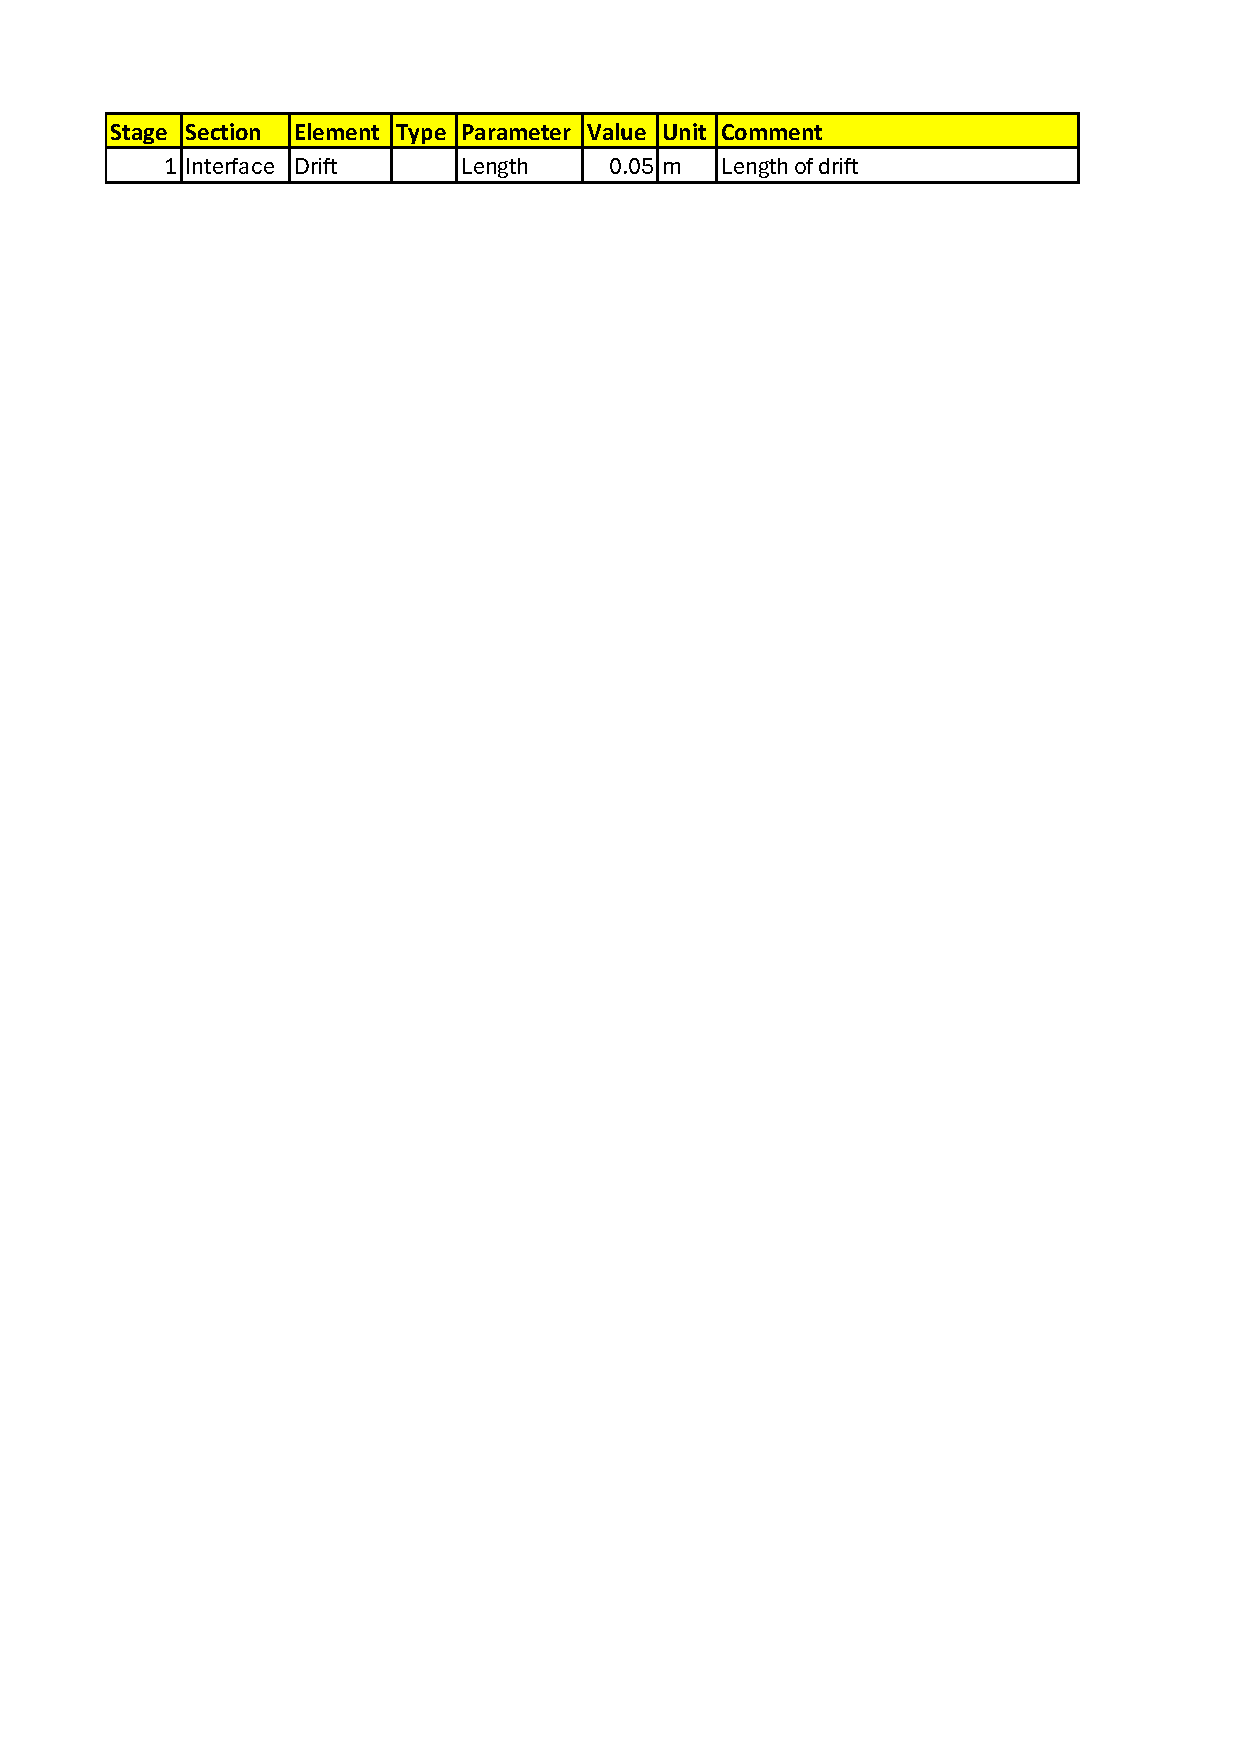
\includegraphics[width=0.95\textwidth]{Drift.pdf}
  \end{center}
\end{table}

\paragraph{Instance attributes and access methods} ~\newline
\label{SubSubSect:Drft:InstAttr}
\noindent
The instance attributes are defined in
table~\ref{Tab:Drft:Attributes}. 
The attributes are accessed and set using the methods defined in
table~\ref{Tab:Drft:Methods}.
\begin{table}[h]
  \caption{
    Definition of attributes of instances of
    the \texttt{Drift(BeamLineElement)} derived class.
    All attributes are required in the call to instantiate the
    element.
  }
  \label{Tab:Drft:Attributes}
  \begin{center}
    \begin{tabular}{|l|c|c|p{10cm}|}
      \hline
      \textbf{Attribute} & \textbf{Type} & \textbf{Unit} & \textbf{Comment}                                                                   \\
      \hline
      \texttt{Length} & float & m & Length of drift. \\
      \hline
    \end{tabular}
  \end{center}
\end{table}
\begin{table}[h]
  \caption{
    Definition of access methods for the \texttt{Facility} derived
    class. 
  }
  \label{Tab:Drft:Methods}
  \begin{center}
    \begin{tabular}{|c|c|p{7cm}|}
      \hline
      \textbf{Set method} & \textbf{Get method}  & \textbf{Comment}                       \\
      \hline
      \texttt{setLength(Length)}   & \texttt{getLength()} & Set/get length of drift (in m). \\
      \texttt{setTransferMatrix()} &                      & Set transfer matrix.            \\
      \hline
    \end{tabular}
  \end{center}
\end{table}

\paragraph{Processing methods} ~\newline
\noindent
The \texttt{Drift} derived class has no processing methods other
than those inheritted from the parent class.

\paragraph{I/o methods} ~\newline
\noindent
The \texttt{Drift} derived class has no i/o methods other than
those inheritted from the parent class.

\paragraph{Utilities} ~\newline
\noindent
The \texttt{Drift} derived class has no utilities other than those
inheritted from the parent class. 

\FloatBarrier

\subsubsection{Derived class: \texttt{Aperture(BeamLineElement)}}

\paragraph{Instantiation} ~\newline
\noindent
The call to instantiate the \texttt{Aperture} derived class is:
\begin{center}
  \texttt{Aperture(Name, rStrt, vStrt, drStrt, dvStrt, ParamList)}
\end{center}
Parent class arguments \texttt{Name}, \texttt{rStrt}, \texttt{vStrt},
\texttt{drStrt}, and \texttt{dvStrt} are described in
section~\ref{SubSubSect:BLE:InstAttr}.
These arguments are passed directly to \texttt{BeamLineElement}.

The lines that specify the \texttt{Aperture} object in the beam-line
specification file are presented in table~\ref{App:MCD:Aprtr:BS}.
\begin{table}[h]
  \caption{
    Entries in the beam-line specification file that define the
    object.
    \texttt{Stage} and \texttt{Section} may be speficied for
    convenience.
    These fields are used in creating the unique string that refers
    to the instance of the derived class.
    The three different types of aperture provided by the derived
    class are instanciated using the entries separarated by solid
    lines.
  }
  \label{App:MCD:Aprtr:BS}
  \begin{center}
    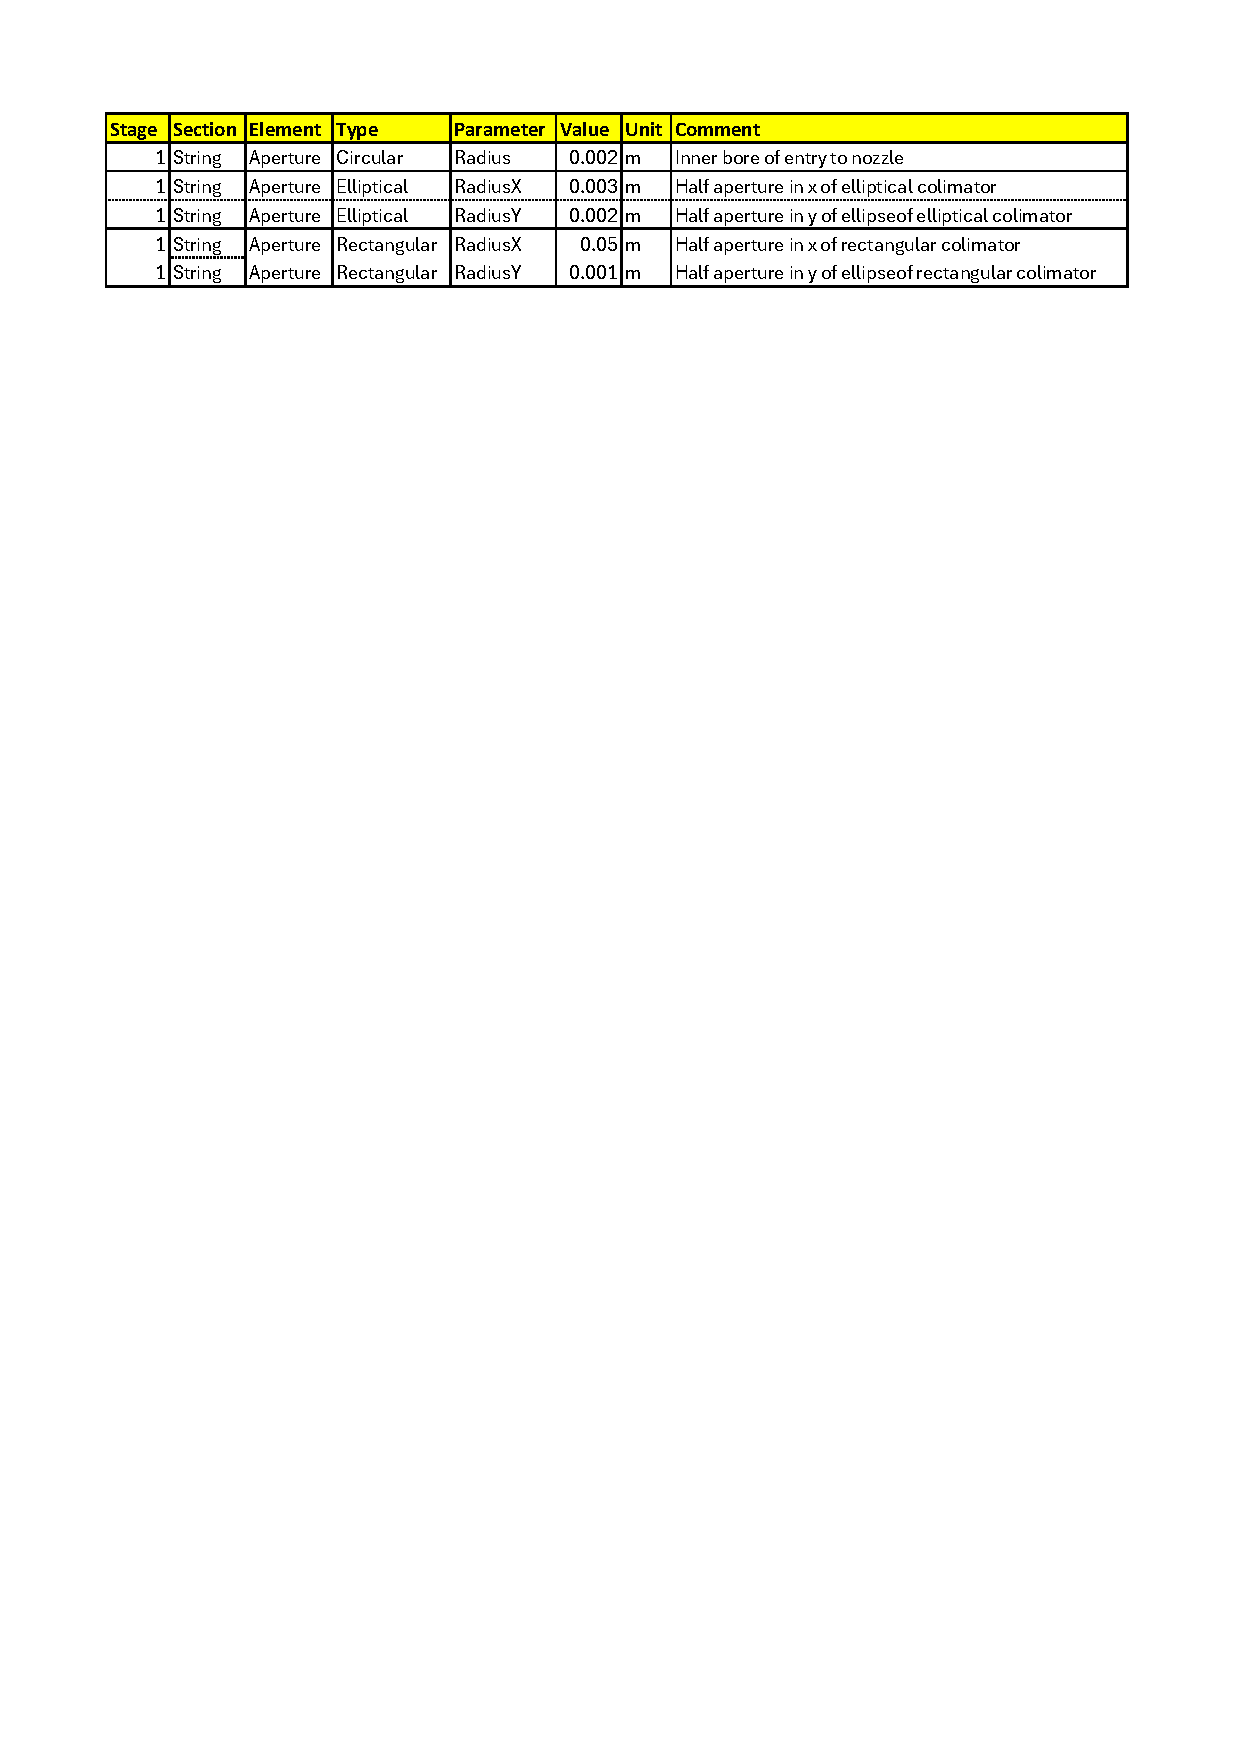
\includegraphics[width=0.95\textwidth]{Aperture.pdf}
  \end{center}
\end{table}

\paragraph{Instance attributes and access methods} ~\newline
\label{SubSubSect:Aprtr:InstAttr}
\noindent
The instance attributes are defined in
table~\ref{Tab:Aprtr:Attributes}. 
The attributes are accessed and set using the methods defined in
table~\ref{Tab:Aprtr:Methods}.
\begin{table}[h]
  \caption{
    Definition of attributes of instances of
    the \texttt{Aperture(BeamLineElement)} derived class.
    All attributes are required in the call to instantiate the
    element.
  }
  \label{Tab:Aprtr:Attributes}
  \begin{center}
    \begin{tabular}{|l|c|c|p{10cm}|}
      \hline
      \textbf{Attribute}   & \textbf{Type} & \textbf{Unit} & \textbf{Comment}                                                                   \\
      \hline
      \texttt{ParamList}   & [] &   & List containing aperture parameters.
                                    The first parameter is an \texttt{int}
                                    and defines the aperture ``\texttt{Type}''.
                                    The remaining elements in the parameter list
                                    are \texttt{float}s with meanings that depend
                                    on \texttt{Type}.                             \\
      \hline
      \texttt{ParamList[0]} & int   &   & \texttt{Type}$=0$; circular                 \\
      \texttt{ParamList[1]} & float & m & Radius of circular aperture                 \\
      \hline
      \texttt{ParamList[0]} & int   &   & \texttt{Type}$=1$; Elliptical                           \\
      \texttt{ParamList[1]} & float & m & Radius of elliptical aperture along $x_{\rm RPLC}$ axis \\
      \texttt{ParamList[2]} & float & m & Radius of elliptical aperture along $y_{\rm RPLC}$ axis \\
      \hline
      \texttt{ParamList[0]} & int   &   & \texttt{Type}$=2$; Rectangular                         \\
      \texttt{ParamList[1]} & float & m & Size of aperture along $x_{\rm RPLC}$ axis \\
      \texttt{ParamList[2]} & float & m & Size of aperture along $y_{\rm RPLC}$ axis \\
      \hline
    \end{tabular}
  \end{center}
\end{table}
\begin{table}[h]
  \caption{
    Definition of access methods for the \texttt{Aperture} derived
    class. 
  }
  \label{Tab:Aprtr:Methods}
  \begin{center}
    \begin{tabular}{|c|c|p{7cm}|}
      \hline
      \textbf{Set method} & \textbf{Get method}  & \textbf{Comment}                                  \\
      \hline
      \texttt{setApertureParameters(ParamList)} &                      & Set aperture parameters.
                                                                         Sets \texttt{Type} and parameters
                                                                         depending on \texttt{Type}. \\
                                                & \texttt{getType()} & Get \texttt{Type} of aperture.\\
                                                & \texttt{getParams()} & Get aperture parameters.    \\
      \hline
    \end{tabular}
  \end{center}
\end{table}

\paragraph{Processing methods} ~\newline
\noindent
The \texttt{Aperture} processing method is defined in
table~\ref{Tab:Aprtr:Methods}.
\begin{table}[h]
  \caption{
    Utilities provided by the \texttt{Aperture} derived
    class. 
  }
  \label{Tab:Aprtr:Methods}
  \begin{center}
    \begin{tabular}{|l|c|c|p{7cm}|}
      \hline
      \textbf{Method} & \textbf{Argument(s)} & \textbf{Return} & \textbf{Comment}                                            \\
      \hline
      \texttt{Transport(V)} & \texttt{np.ndarray} & \texttt{np.ndarray} or \texttt{None} &
                        Transport trace-space vector \texttt{V}.  If \texttt{V} falls outside of the aperture, return \texttt{None}. \\
      \hline
    \end{tabular}
  \end{center}
\end{table}

\FloatBarrier

\paragraph{I/o methods} ~\newline
\noindent
The \texttt{Aperture} derived class has no i/o methods other than
those inheritted from the parent class.

\paragraph{Utilities} ~\newline
\noindent
The \texttt{Aperture} derived class has no utilities other than those
inheritted from the parent class. 

\subsubsection{Derived class: \texttt{FocusQuadrupole(BeamLineElement)}}

\paragraph{Instantiation} ~\newline
\noindent
The call to instantiate the \texttt{FocusQuadrupole} derived class is:
\begin{center}
  \texttt{FocusQuadrupole(Name, rStrt, vStrt, drStrt, dvStrt, Length,
          Strength, kFQ)} 
\end{center}
Parent class arguments \texttt{Name}, \texttt{rStrt}, \texttt{vStrt},
\texttt{drStrt}, and \texttt{dvStrt} are described in
section~\ref{SubSubSect:BLE:InstAttr}.
These arguments are passed directly to \texttt{BeamLineElement}.
The quadrupole \texttt{Length} is required together with
either the field gradient, \texttt{Strength}
(equation~\ref{Eq:Trnsf:gxy}), or the quadrupole $k$
parameter, \texttt{kFQ} (equation~\ref{Eq:Effectivekq}).

The lines that specify the \texttt{FocusQuadrupole} object in the
beam-line specification file are presented in
table~\ref{App:MCD:Quads:BS}. 
\begin{table}[h]
  \caption{
    Entries in the beam-line specification file that define the
    object.
    \texttt{Stage} and \texttt{Section} may be speficied for
    convenience.
    These fields are used in creating the unique string that refers
    to the instance of the derived class.
    The entries that define focus quadrupole are shaded light grey
    while the lines that define the defocus quadrupole are shaded in a
    darker shade of grey.
  }
  \label{App:MCD:Quads:BS}
  \begin{center}
    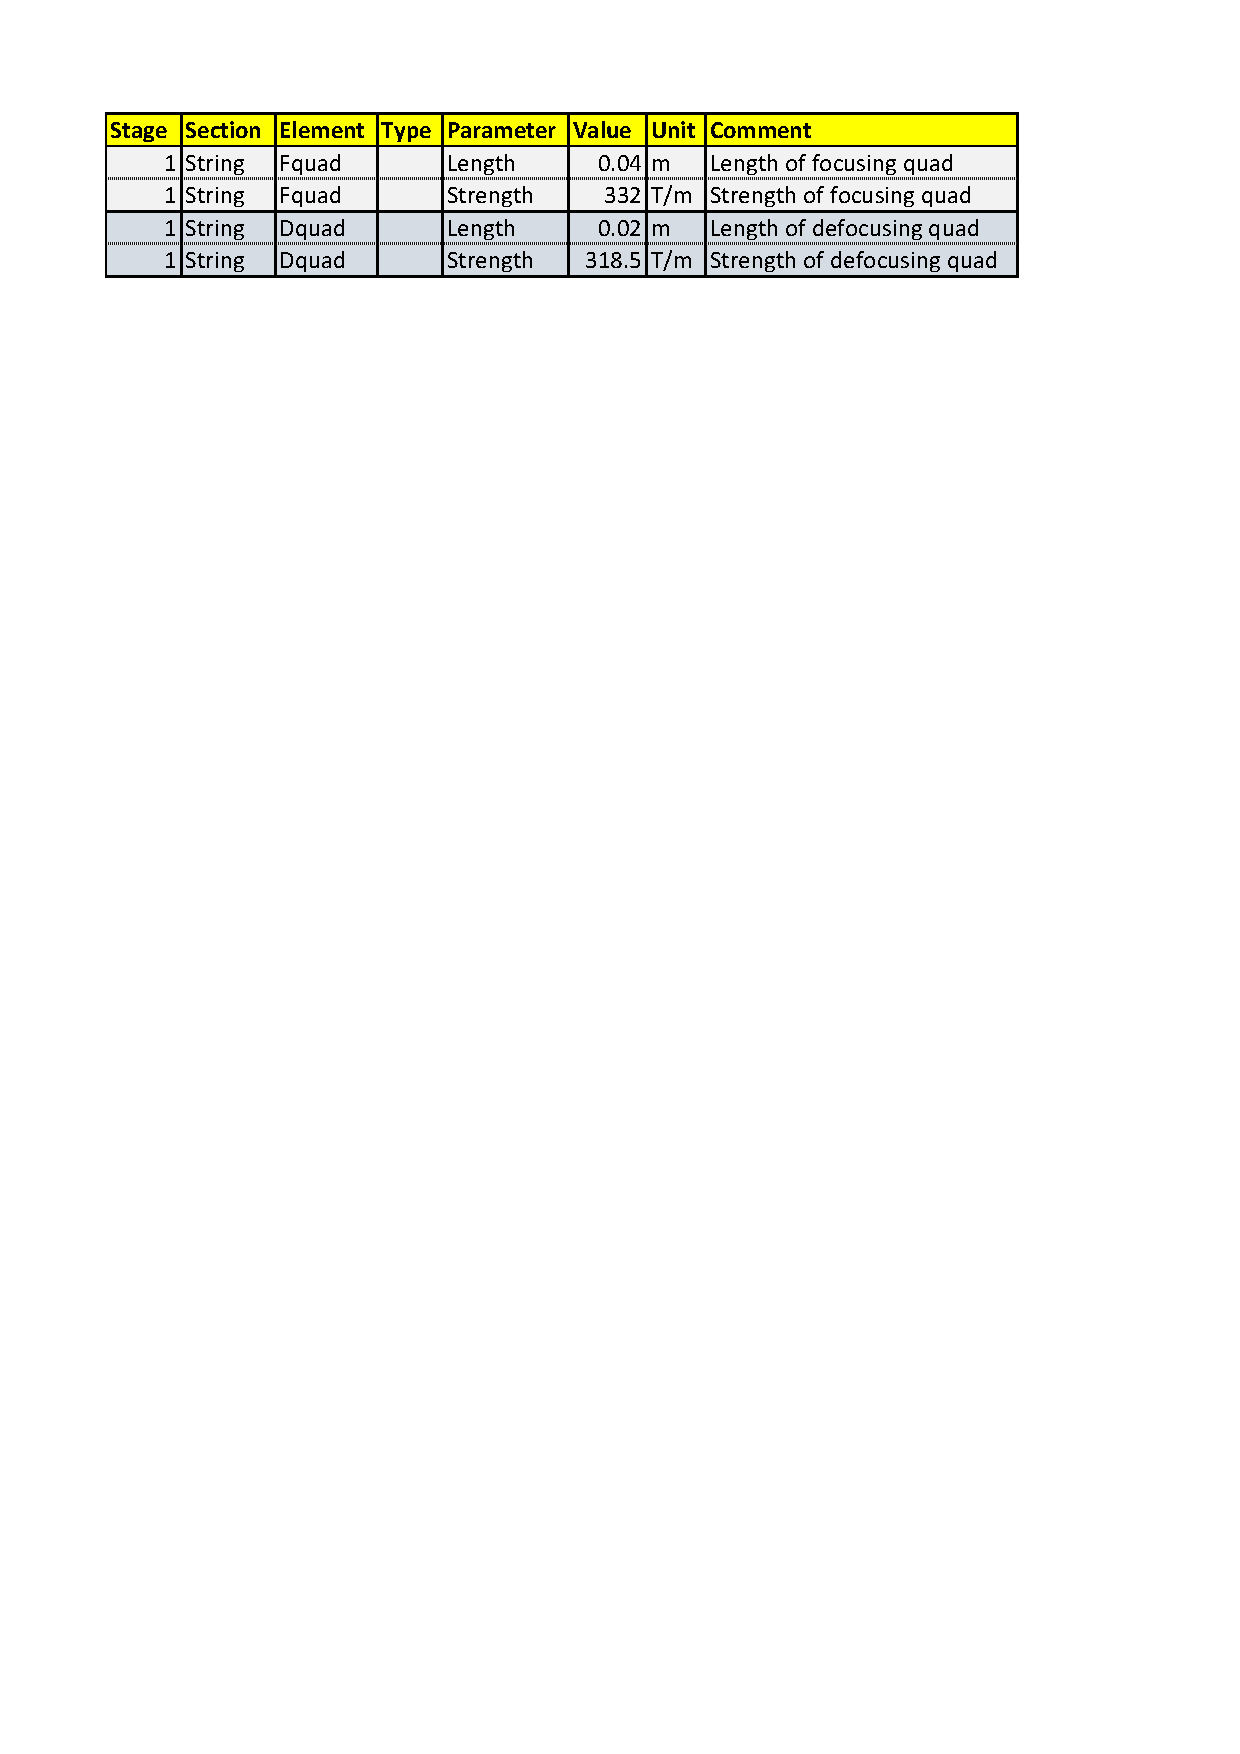
\includegraphics[width=0.95\textwidth]{Quads.pdf}
  \end{center}
\end{table}

\paragraph{Instance attributes and access methods} ~\newline
\label{SubSubSect:FQuad:InstAttr}
\noindent
The instance attributes are defined in
table~\ref{Tab:FQuad:Attributes}. 
The attributes are accessed and set using the methods defined in
table~\ref{Tab:FQuad:Methods}.
\begin{table}[h]
  \caption{
    Definition of attributes of instances of
    the \texttt{FocusQuadrupole(BeamLineElement)} derived class.
    All attributes are required in the call to instantiate the
    element.
  }
  \label{Tab:FQuad:Attributes}
  \begin{center}
    \begin{tabular}{|l|c|c|p{10cm}|}
      \hline
      \textbf{Attribute}   & \textbf{Type} & \textbf{Unit} & \textbf{Comment}                    \\
      \hline
      \texttt{FQmode}   & int   &       & If 0, use particle momentum in calculation of transfer
                                          matrix; if 1, use reference particle momentum.         \\
      \texttt{Length}   & float & m     & Effective length of quadrupole.                        \\
      \texttt{Strength} & float & T/m   & Magnetic field gradient; required if kFQ is not given. \\
      \texttt{kFQ}      & float & m$^{-2}$ & Quadrupole $k$ parameter.                               \\
      \hline
    \end{tabular}
  \end{center}
\end{table}
\begin{table}[h]
  \caption{
    Definition of access methods for the \texttt{FocusQuadrupole} derived
    class. 
  }
  \label{Tab:FQuad:Methods}
  \begin{center}
    \begin{tabular}{|c|c|p{7cm}|}
      \hline
      \textbf{Set method} & \textbf{Get method}  & \textbf{Comment}                                    \\
      \hline
      \texttt{setFQmode(FQmode)}   & \texttt{getFQmode()}   & Set/get FQmode.                        \\
      \texttt{setLength(Length)}   & \texttt{getLength()}   & Set/get length.                        \\
      \texttt{setStrength(Length)} & \texttt{getStrength()} & Set/get strength (field gradient).     \\
      \texttt{setKFQ(Length)}      & \texttt{getKFQ()}      & Set/get kFQ, quadrupole $k$ parameter. \\
      \hline
    \end{tabular}
  \end{center}
\end{table}

\paragraph{Processing methods} ~\newline
\noindent
The \texttt{FocusQuadrupole} processing methods are defined in
table~\ref{Tab:FQuad:Methods}.
\begin{table}[h]
  \caption{
    Utilities provided by the \texttt{FocusQuadrupole} derived
    class. 
  }
  \label{Tab:FQuad:Methods}
  \begin{center}
    \begin{tabular}{|l|c|c|p{7cm}|}
      \hline
      \textbf{Method} & \textbf{Argument(s)} & \textbf{Return} & \textbf{Comment}                     \\
      \hline
      \texttt{calckFQ()} &  & float & Calculates \texttt{kFQ} if strength is given in instance attributes. \\
      \texttt{calcStrength()} &  & float & Calculates \texttt{Strength} if \texttt{kFQ} is is given in instance attributes. \\
      \hline
    \end{tabular}
  \end{center}
\end{table}

\paragraph{I/o methods} ~\newline
\noindent
The \texttt{Focusquadrupole} derived class has no i/o methods other than
those inheritted from the parent class.

\paragraph{Utilities} ~\newline
\noindent
The \texttt{Focusquadrupole} derived class has no utilities other than those
inheritted from the parent class. 

%\FloatBarrier

\subsubsection{Derived class: \texttt{DefocusQuadrupole(BeamLineElement)}}

\paragraph{Instantiation} ~\newline
\noindent
The call to instantiate the \texttt{DefocusQuadrupole} derived class is:
\begin{center}
  \texttt{DefocusQuadrupole(Name, rStrt, vStrt, drStrt, dvStrt, Length,
          Strength, kDQ)} 
\end{center}
Parent class arguments \texttt{Name}, \texttt{rStrt}, \texttt{vStrt},
\texttt{drStrt}, and \texttt{dvStrt} are described in
section~\ref{SubSubSect:BLE:InstAttr}.
These arguments are passed directly to \texttt{BeamLineElement}.
The quadrupole \texttt{Length} is required together with
either the field gradient, \texttt{Strength}
(equation~\ref{Eq:Trnsf:gxy}), or the quadrupole $k$
parameter, \texttt{kDQ} (equation~\ref{Eq:Effectivekq}).

The lines that specify the \texttt{FocusQuadrupole} object in the
beam-line specification file are presented in
table~\ref{App:MCD:Quads:BS}.

\paragraph{Instance attributes and access methods} ~\newline
\label{SubSubSect:DQuad:InstAttr}
\noindent
The instance attributes are defined in
table~\ref{Tab:DQuad:Attributes}. 
The attributes are accessed and set using the methods defined in
table~\ref{Tab:DQuad:Methods}.
\begin{table}[h]
  \caption{
    Definition of attributes of instances of
    the \texttt{DefocusQuadrupole(BeamLineElement)} derived class.
    All attributes are required in the call to instantiate the
    element.
  }
  \label{Tab:DQuad:Attributes}
  \begin{center}
    \begin{tabular}{|l|c|c|p{10cm}|}
      \hline
      \textbf{Attribute}   & \textbf{Type} & \textbf{Unit} & \textbf{Comment}                    \\
      \hline
      \texttt{DQmode}   & int   &       & If 0, use particle momentum in calculation of transfer
                                          matrix; if 1, use reference particle momentum.         \\
      \texttt{Length}   & float & m     & Effective length of quadrupole.                        \\
      \texttt{Strength} & float & T/m   & Magnetic field gradient; required if kDQ is not given. \\
      \texttt{kDQ}      & float & m$^{-2}$ & Quadrupole $k$ parameter.                               \\
      \hline
    \end{tabular}
  \end{center}
\end{table}
\begin{table}[h]
  \caption{
    Definition of access methods for the \texttt{DefocusQuadrupole} derived
    class. 
  }
  \label{Tab:DQuad:Methods}
  \begin{center}
    \begin{tabular}{|c|c|p{7cm}|}
      \hline
      \textbf{Set method} & \textbf{Get method}  & \textbf{Comment}                                    \\
      \hline
      \texttt{setDQmode(DQmode)}   & \texttt{getDQmode()}   & Set/get DQmode.                        \\
      \texttt{setLength(Length)}   & \texttt{getLength()}   & Set/get length.                        \\
      \texttt{setStrength(Length)} & \texttt{getStrength()} & Set/get strength (field gradient).     \\
      \texttt{setKDQ(Length)}      & \texttt{getKDQ()}      & Set/get kDQ, quadrupole $k$ parameter. \\
      \hline
    \end{tabular}
  \end{center}
\end{table}

\paragraph{Processing methods} ~\newline
\noindent
The \texttt{DefocusQuadrupole} processing methods are defined in
table~\ref{Tab:DQuad:Methods}.
\begin{table}[h]
  \caption{
    Utilities provided by the \texttt{DefocusQuadrupole} derived
    class. 
  }
  \label{Tab:DQuad:Methods}
  \begin{center}
    \begin{tabular}{|l|c|c|p{7cm}|}
      \hline
      \textbf{Method} & \textbf{Argument(s)} & \textbf{Return} & \textbf{Comment}                     \\
      \hline
      \texttt{calckDQ()} &  & float & Calculates \texttt{kDQ} if strength is specified.               \\
      \texttt{calcStrength()} &  & float & Calculates \texttt{Strength} if \texttt{kDQ} is specified. \\
      \hline
    \end{tabular}
  \end{center}
\end{table}

\paragraph{I/o methods} ~\newline
\noindent
The \texttt{Defocusquadrupole} derived class has no i/o methods other
than those inheritted from the parent class.

\paragraph{Utilities} ~\newline
\noindent
The \texttt{Defocusquadrupole} derived class has no utilities other
than those inheritted from the parent class. 

\FloatBarrier

\subsubsection{Derived class: \texttt{SectorDipole(BeamLineElement)}}

\paragraph{Instantiation} ~\newline
\noindent
The call to instantiate the \texttt{SectorDipole} derived class is:
\begin{center}
  \texttt{SectorDipole(Name, rStrt, vStrt, drStrt, dvStrt, 
          Angle, B)} 
\end{center}
Parent class arguments \texttt{Name}, \texttt{rStrt}, \texttt{vStrt},
\texttt{drStrt}, and \texttt{dvStrt} are described in
section~\ref{SubSubSect:BLE:InstAttr}.
These arguments are passed directly to \texttt{BeamLineElement}.

The lines that specify the \texttt{SectorDipole} object in the
beam-line specification file are presented in
table~\ref{App:MCD:SctrDpl:BS}. 
\begin{table}[h]
  \caption{
    Entries in the beam-line specification file that define the
    sector dipole object.
    \texttt{Stage} and \texttt{Section} may be speficied for
    convenience.
    These fields are used in creating the unique string that refers
    to the instance of the derived class.
  }
  \label{App:MCD:SctrDpl:BS}
  \begin{center}
    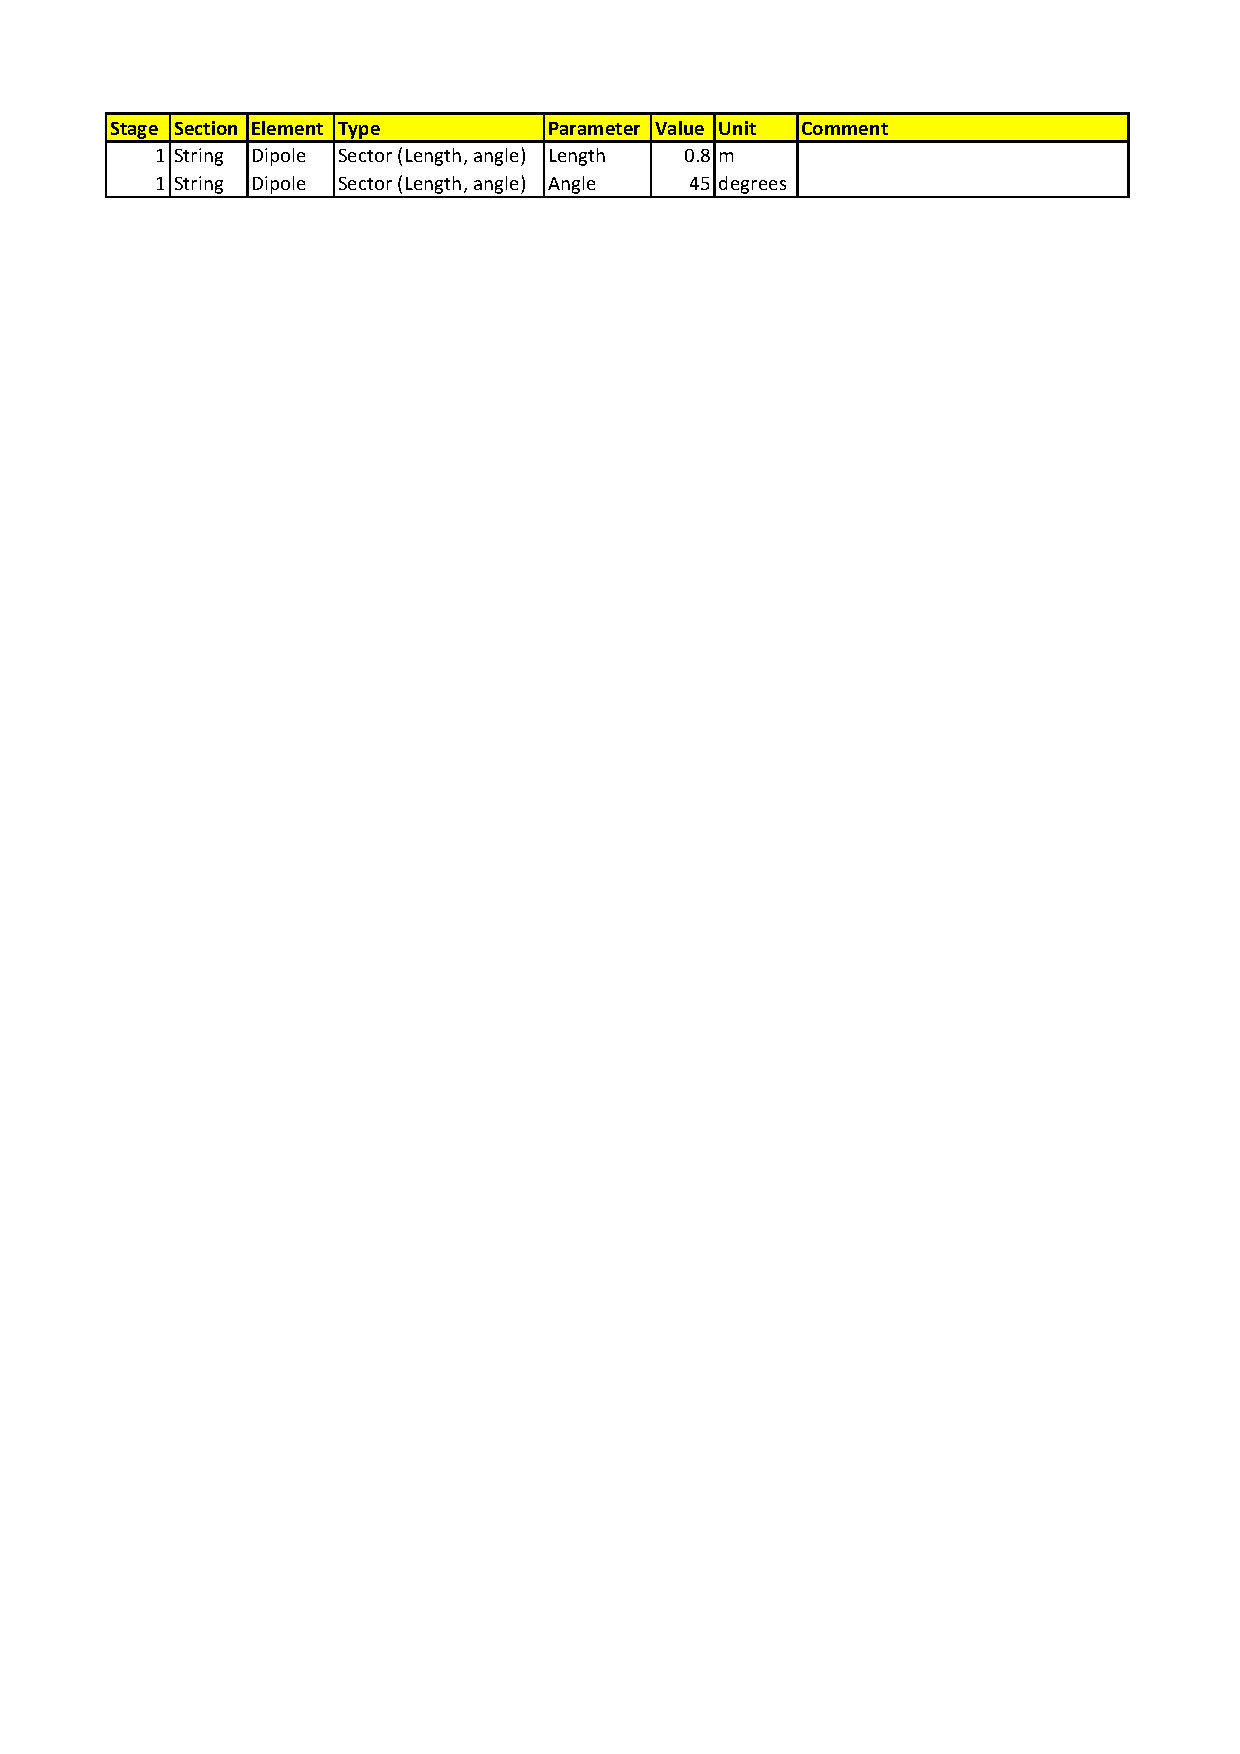
\includegraphics[width=0.95\textwidth]{Dipole.pdf}
  \end{center}
\end{table}

The orientation of the RLPC coordinate axes with respect to those of
the laboratory frame changes from the start of sector dipole to its
end.
Referring to figure~\ref{fig:Dipole}, the vector, $\bm{v}_{\rm ES}$,
that translates the origin of the RLPC coordinate system at the start
of the sector dipole to the origin of the RLPC coordinate system at
its end is given by:
\begin{equation}
  \bm{v}_{\rm ES} = 2 \rho_0 \sin\left( \frac{\phi}{2} \right)
                     \begin{pmatrix}
                       \sin\left( \frac{\phi}{2} \right) \\
                       0                                 \\
                       \cos\left( \frac{\phi}{2} \right)
                     \end{pmatrix} \,;
\end{equation}
where $\rho_0$ is the radius of the circular locus of the trajectory
of the reference particle.
If the rotation matrix taking the RPLC axes at the start of the sector
dipole to the laboratory coordinate axes is
$\underline{\underline{R}}_{\rm S}$, then the vector,
$\bm{v}^{\rm lab}_{\rm ES}$, that translates from the start 
of the sector dipole to its end in laboratory coordinates is given by:
\begin{equation}
  \bm{v}^{\rm lab}_{\rm ES} = \underline{\underline{R}}_{\rm S} \bm{v}_{\rm ES} \,.
\end{equation}
The rotation matrix that transforms from the RPLC system at the end
of the sector dipole to the laboratory coordinate system,
$\underline{\underline{R}}_{\rm E}$ is given by:
\begin{equation}
  \underline{\underline{R}}_{\rm E} =
      \underline{\underline{R}}_{\rm S} \underline{\underline{R}} \, ;
\end{equation}
where:
\begin{equation}
  \underline{\underline{R}} = 
        \begin{pmatrix}
          \cos \phi & 0 & -\sin \phi \\
          0         & 1 &  0         \\
          \sin \phi & 0 &  \cos \phi 
        \end{pmatrix} \, .
\end{equation}

\paragraph{Instance attributes and access methods} ~\newline
\label{SubSubSect:SDpl:InstAttr}
\noindent
The instance attributes are defined in
table~\ref{Tab:SDpl:Attributes}. 
The attributes are accessed and set using the methods defined in
table~\ref{Tab:SDpl:Methods}.
\begin{table}[h]
  \caption{
    Definition of attributes of instances of
    the \texttt{SectorDipole(BeamLineElement)} derived class.
    All attributes are required in the call to instantiate the
    element.
  }
  \label{Tab:SDpl:Attributes}
  \begin{center}
    \begin{tabular}{|l|c|c|p{10cm}|}
      \hline
      \textbf{Attribute}   & \textbf{Type} & \textbf{Unit} & \textbf{Comment}                      \\
      \hline
      \texttt{Angle}   & float & rad & Angle through which sector dipole bends positive reference
                                 particle.                                                         \\
      \texttt{B}       & float & T   & Magnetic field.                                             \\
      \hline
    \end{tabular}
  \end{center}
\end{table}
\begin{table}[h]
  \caption{
    Definition of access methods for the \texttt{SectorDipole} derived
    class. 
  }
  \label{Tab:SDpl:Methods}
  \begin{center}
    \begin{tabular}{|c|c|p{7cm}|}
      \hline
      \textbf{Set method} & \textbf{Get method}  & \textbf{Comment}       \\
      \hline
      \texttt{setAngle(Angle)}     & \texttt{getAngle()}  & Set/get bending angle.         \\
      \texttt{setB(B)}             & \texttt{getB()}      & Set/get dipole magnetic field. \\
      \texttt{setLength()}         & \texttt{getLength()} & Set/get length of reference
                                                            particle trajectory through
                                                            sector dipole (arc length).    \\
      \hline
    \end{tabular}
  \end{center}
\end{table}

\paragraph{Processing methods} ~\newline
\noindent
The \texttt{SectorDipole} derived class has no processing methods
other than those inheritted from the parent class.

\paragraph{I/o methods} ~\newline
\noindent
The \texttt{SectorDipole} derived class has no i/o methods other
than those inheritted from the parent class.

\paragraph{Utilities} ~\newline
\noindent
The \texttt{SectorDipole} derived class has no utilities other
than those inheritted from the parent class. 

\FloatBarrier

\subsubsection{Derived class: \texttt{Solenoid(BeamLineElement)}}

\paragraph{Instantiation} ~\newline
\noindent
The call to instantiate the \texttt{Solenoid} derived class is:
\begin{center}
  \texttt{Solenoid(Name, rStrt, vStrt, drStrt, dvStrt,
          Length, Strength, kSol)} 
\end{center}
Parent class arguments \texttt{Name}, \texttt{rStrt}, \texttt{vStrt},
\texttt{drStrt}, and \texttt{dvStrt} are described in
section~\ref{SubSubSect:BLE:InstAttr}.
These arguments are passed directly to \texttt{BeamLineElement}.
The solenoid \texttt{Length} is required together with either the
magnetic field strength, \texttt{Strength} or the solenoid $k$
parameter, \texttt{kSol} (equation~\ref{Eq:Effectiveks}).  

The lines that specify the \texttt{Solenoid} object in the
beam-line specification file are presented in
table~\ref{App:MCD:Slnd:BS}. 
\begin{table}[h]
  \caption{
    Entries in the beam-line specification file that define the
    solenoid object.
    \texttt{Stage} and \texttt{Section} may be speficied for
    convenience.
    These fields are used in creating the unique string that refers
    to the instance of the derived class.
  }
  \label{App:MCD:Slnd:BS}
  \begin{center}
    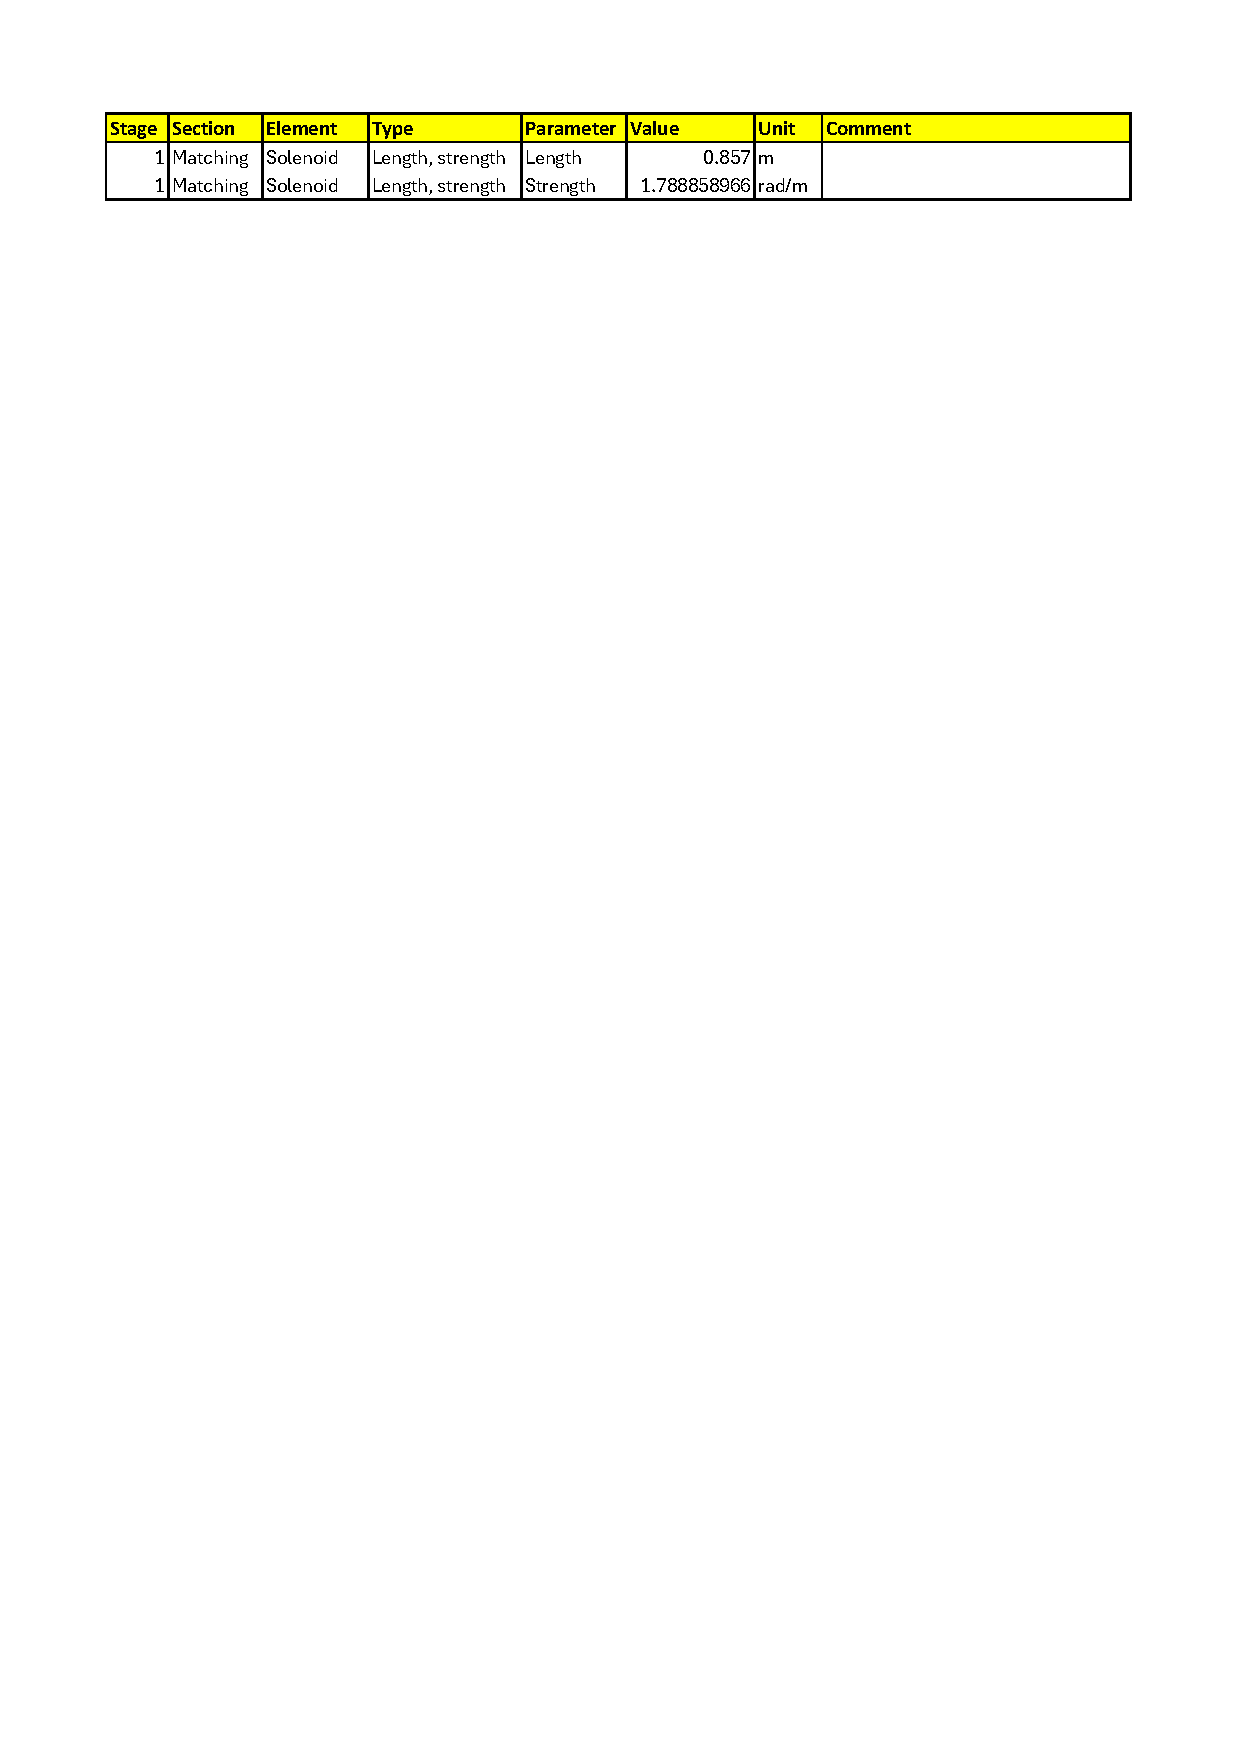
\includegraphics[width=0.95\textwidth]{Solenoid.pdf}
  \end{center}
\end{table}

\paragraph{Instance attributes and access methods} ~\newline
\label{SubSubSect:Slnd:InstAttr}
\noindent
The instance attributes are defined in
table~\ref{Tab:Slnd:Attributes}. 
The attributes are accessed and set using the methods defined in
table~\ref{Tab:Slnd:Methods}.
\begin{table}[h]
  \caption{
    Definition of attributes of instances of
    the \texttt{Solenoid(BeamLineElement)} derived class.
    All attributes are required in the call to instantiate the
    element.
  }
  \label{Tab:Slnd:Attributes}
  \begin{center}
    \begin{tabular}{|l|c|c|p{10cm}|}
      \hline
      \textbf{Attribute}   & \textbf{Type} & \textbf{Unit} & \textbf{Comment}                     \\
      \hline
      \texttt{Length}   & float & m     & Effective length of solenoid.                           \\
      \texttt{Strength} & float & T/m   & Magnetic field gradient; required if kSol is not given. \\
      \texttt{kSol}     & float & m$^{-2}$ & GaborLens $k$ parameter required if \texttt{Strength}
                                          not given.                                              \\
      \hline
    \end{tabular}
  \end{center}
\end{table}
\begin{table}[h]
  \caption{
    Definition of access methods for the \texttt{Solenoid} derived
    class. 
  }
  \label{Tab:Slnd:Methods}
  \begin{center}
    \begin{tabular}{|c|c|p{7cm}|}
      \hline
      \textbf{Set method} & \textbf{Get method}  & \textbf{Comment}                                  \\
      \hline
      \texttt{setLength(Length)}   & \texttt{getLength()}   & Set/get length.                        \\
      \texttt{setStrength(B)}      & \texttt{getStrength()} & Set/get strength (solenoid magnetic
                                                              field).                                \\
      \texttt{setKSol(Length)}     & \texttt{getKFQ()}      & Set/get kSol, solenoid $k$ parameter.  \\
      \hline
    \end{tabular}
  \end{center}
\end{table}

\paragraph{Processing methods} ~\newline
\noindent
The \texttt{Solenoid} processing method is defined in
table~\ref{Tab:Slnd:Methods}.

\paragraph{I/o methods} ~\newline
\noindent
The \texttt{Solenoid} derived class has no i/o methods other
than those inheritted from the parent class.

\paragraph{Utilities} ~\newline
\noindent
The \texttt{Solenoid} derived class has no utilities other
than those inheritted from the parent class. 

\begin{table}[h]
  \caption{
    Utilities provided by the \texttt{Solenoid} derived
    class. 
  }
  \label{Tab:Slnd:Methods}
  \begin{center}
    \begin{tabular}{|l|c|c|p{7cm}|}
      \hline
      \textbf{Method} & \textbf{Argument(s)} & \textbf{Return} & \textbf{Comment}                      \\
      \hline
      \texttt{calckSol()}     &  & float & Calculates \texttt{kSol} if strength is specified.          \\
      \texttt{calcStrength()} &  & float & Calculates \texttt{Strength} if \texttt{kSol} is specified. \\
      \hline
    \end{tabular}
  \end{center}
\end{table}

\subsubsection{Derived class: \texttt{GaborLens(BeamLineElement)}}

\paragraph{Instantiation} ~\newline
\noindent
The call to instantiate the \texttt{GaborLens} derived class is:
\begin{center}
  \texttt{GaborLens(Name, rStrt, vStrt, drStrt, dvStrt,
          Bz, VA, RA, Rp, Length, kSol)}
\end{center}
Parent class arguments \texttt{Name}, \texttt{rStrt}, \texttt{vStrt},
\texttt{drStrt}, and \texttt{dvStrt} are described in
section~\ref{SubSubSect:BLE:InstAttr}.
These arguments are passed directly to \texttt{BeamLineElement}.
The Gabor lens \texttt{Length} is required together with either the
parameters \texttt{Bz}, \texttt{VA}, \texttt{RA}, and \texttt{Rp}
corresponding, respectively, to the parameters $B_z$, $V_A$, $V_A$ and
$R_p$ defined in section~\ref{SubSect:TrnsFrMtrx:GL}, or $kSol$, the
solenoid strength parameter of the equaivalent solenoid (see
section~\ref{SubSect:TrnsFrMtrx:GL}).
The effective electon number density inside the trap is calculated
using either \texttt{Bz}, \texttt{VA}, \texttt{RA} and \texttt{Rp}
or \texttt{kSol}.

The lines that specify the \texttt{GaborLens} object in the
beam-line specification file are presented in
table~\ref{App:MCD:Slnd:BS}. 
\begin{table}[h]
  \caption{
    Entries in the beam-line specification file that define the
    Gabor lens object.
    \texttt{Stage} and \texttt{Section} may be speficied for
    convenience.
    These fields are used in creating the unique string that refers
    to the instance of the derived class.
  }
  \label{App:MCD:Slnd:BS}
  \begin{center}
    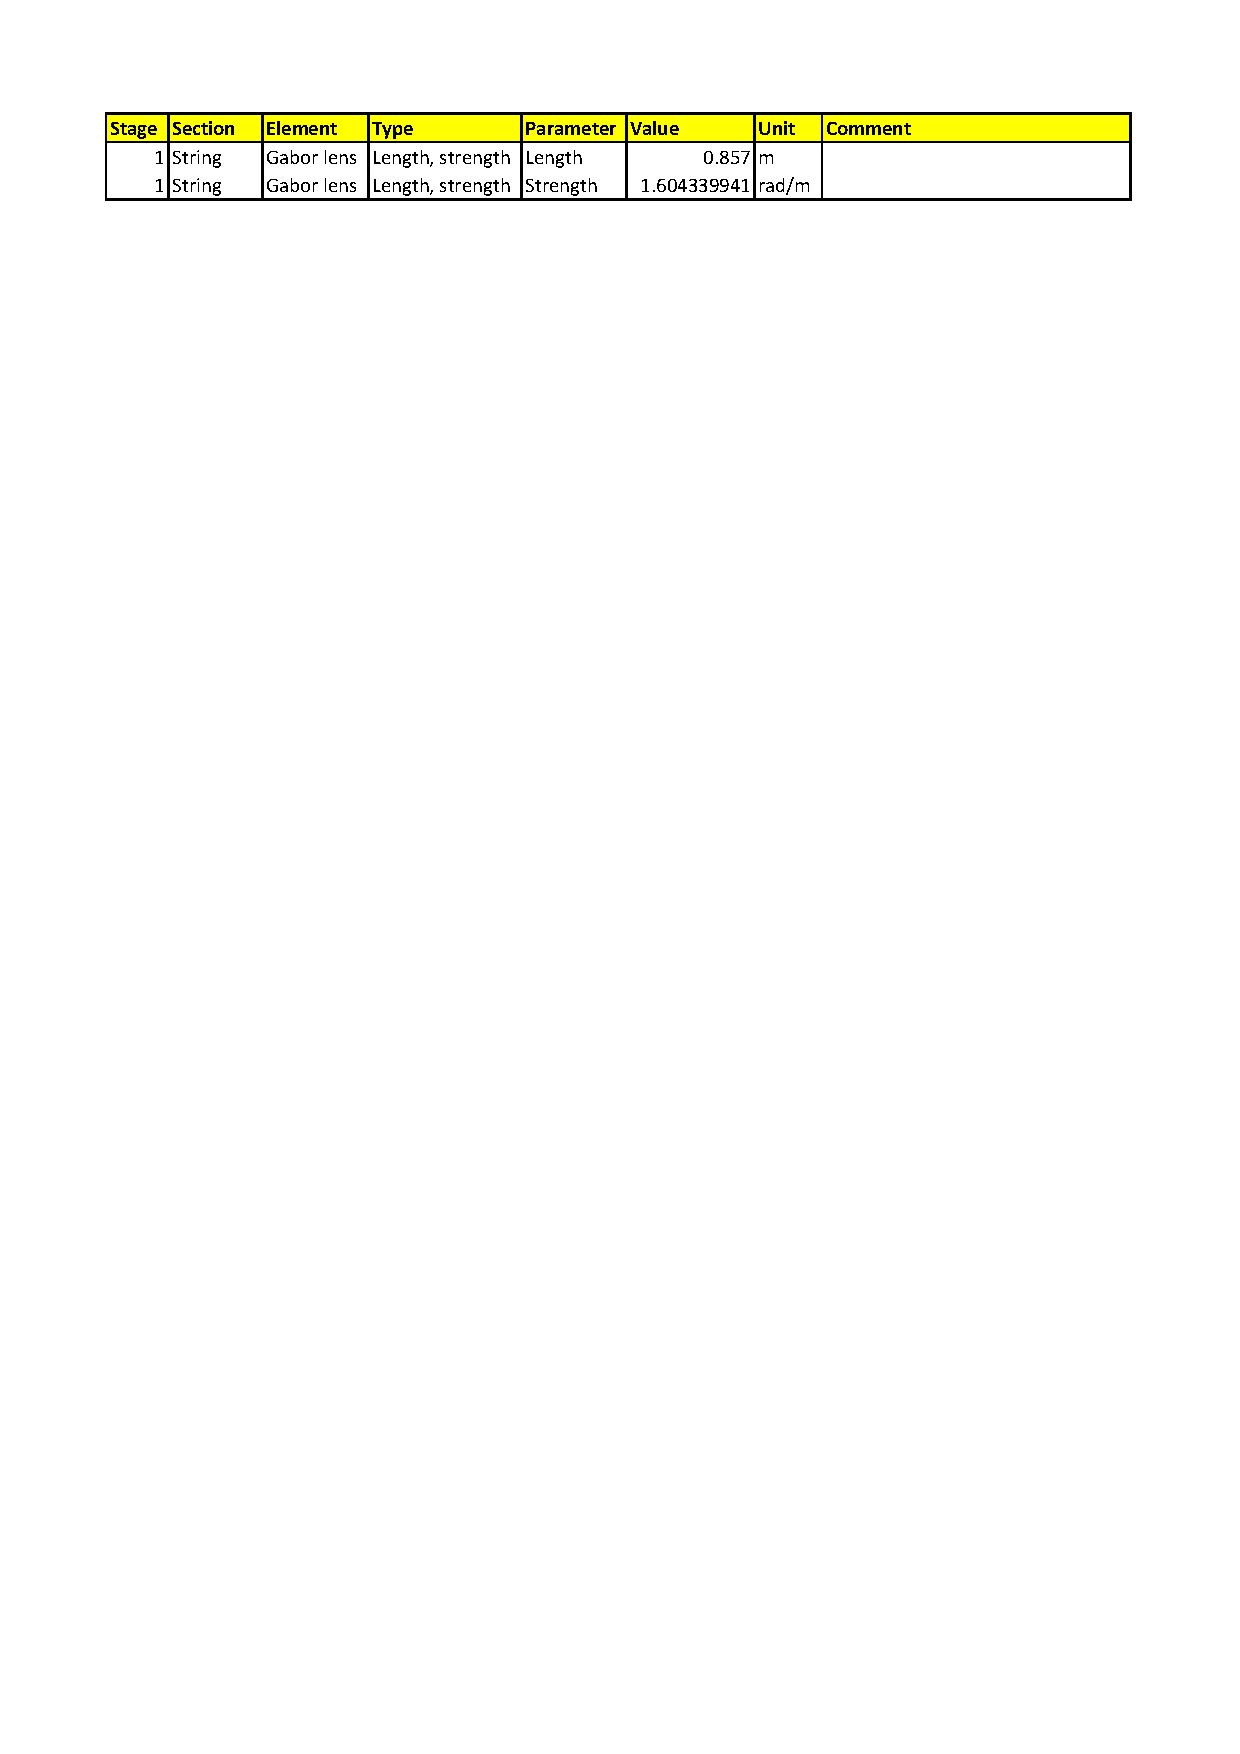
\includegraphics[width=0.95\textwidth]{Gabor.pdf}
  \end{center}
\end{table}

\paragraph{Instance attributes and access methods} ~\newline
\label{SubSubSect:GbrLns:InstAttr}
\noindent
The instance attributes are defined in
table~\ref{Tab:GbrLns:Attributes}. 
The attributes are accessed and set using the methods defined in
table~\ref{Tab:GbrLns:Methods}.
\begin{table}[h]
  \caption{
    Definition of attributes of instances of
    the \texttt{GaborLens(BeamLineElement)} derived class.
    All attributes are required in the call to instantiate the
    element.
  }
  \label{Tab:GbrLns:Attributes}
  \begin{center}
    \begin{tabular}{|l|c|c|p{10cm}|}
      \hline
      \textbf{Attribute}   & \textbf{Type} & \textbf{Unit} & \textbf{Comment}                    \\
      \hline
      \texttt{Bz}   & float & T     & Effective length of Gabor lens.                            \\
      \texttt{VA}   & float & V     & Effective length of Gabor lens.                            \\
      \texttt{RA}   & float & m     & Effective length of Gabor lens.                            \\
      \texttt{RP}   & float & m     & Effective length of Gabor lens.                            \\
      \texttt{Length}   & float & m     & Effective length of Gabor lens.                         \\
      \texttt{Strength} & float & T/m   & Magnetic field gradient; required if kSol is not given. \\
      \texttt{kSol}     & float & m$^{-2}$ & $k$ parameter of the solenoid with the equivalent
                                            focusing strength.                                    \\
      \hline
    \end{tabular}
  \end{center}
\end{table}
\begin{table}[h]
  \caption{
    Definition of access methods for the \texttt{GaborLens} derived
    class. 
  }
  \label{Tab:GbrLns:Methods}
  \begin{center}
    \begin{tabular}{|c|c|p{7cm}|}
      \hline
      \textbf{Set method} & \textbf{Get method}  & \textbf{Comment}                                                 \\
      \hline
      \texttt{setBz(Bz)}         & \texttt{getBz()}     & Set/get magnetic field of the Penning-Malmberg trap.      \\
      \texttt{setVA(VA)}         & \texttt{getVA()}     & Set/get anode voltage of the Penning-Malmberg trap.       \\
      \texttt{setRA(RA)}         & \texttt{getRA()}     & Set/get radius of the anode of the Penning-Malmberg trap. \\
      \texttt{setRP(RP)}         & \texttt{getRP()}     & Set/get magnetic effective radiius of the plasma confined 
                                                          within the Penning-Malmberg trap.                         \\
      \texttt{setLength(Length)} & \texttt{getLength()} & Set/get effective length of the lens.                     \\

      \texttt{setStrength(Strength)} & \texttt{getStrength()} & Set/get k-parameter of the solenoid with the
                                                                equivalent focal length.                            \\
      \texttt{setElectronDenisty()} & \texttt{getElectronDenisty()} & Set/get electron density.                     \\
      \hline
    \end{tabular}
  \end{center}
\end{table}

\paragraph{Processing methods} ~\newline
\noindent
The \texttt{GaborLens} processing method is defined in
table~\ref{Tab:Slnd:Methods}.

\paragraph{I/o methods} ~\newline
\noindent
The \texttt{GaborLens} derived class has no i/o methods other
than those inheritted from the parent class.

\paragraph{Utilities} ~\newline
\noindent
The \texttt{GaborLens} derived class has no utilities other
than those inheritted from the parent class. 

\FloatBarrier

\subsubsection{Derived class: \texttt{CylindricalRFCavity(BeamLineElement)}}

\paragraph{Instantiation} ~\newline
\noindent
The call to instantiate the \texttt{CylindricalRFCavity} derived class is:
\begin{center}
  \texttt{CylindricalRFCavity(Name, rStrt, vStrt, drStrt, dvStrt,
          Gradient, Frequency, Phase)}
\end{center}
Parent class arguments \texttt{Name}, \texttt{rStrt}, \texttt{vStrt},
\texttt{drStrt}, and \texttt{dvStrt} are described in
section~\ref{SubSubSect:BLE:InstAttr}.
These arguments are passed directly to \texttt{BeamLineElement}.

The lines that specify the \texttt{CylindricalCavity} object in the
beam-line specification file are presented in
table~\ref{App:MCD:CylCav:BS}. 
\begin{table}[h]
  \caption{
    Entries in the beam-line specification file that define the
    cylindrical-cavity object.
    \texttt{Stage} and \texttt{Section} may be speficied for
    convenience.
    These fields are used in creating the unique string that refers
    to the instance of the derived class.
  }
  \label{App:MCD:CylCav:BS}
  \begin{center}
    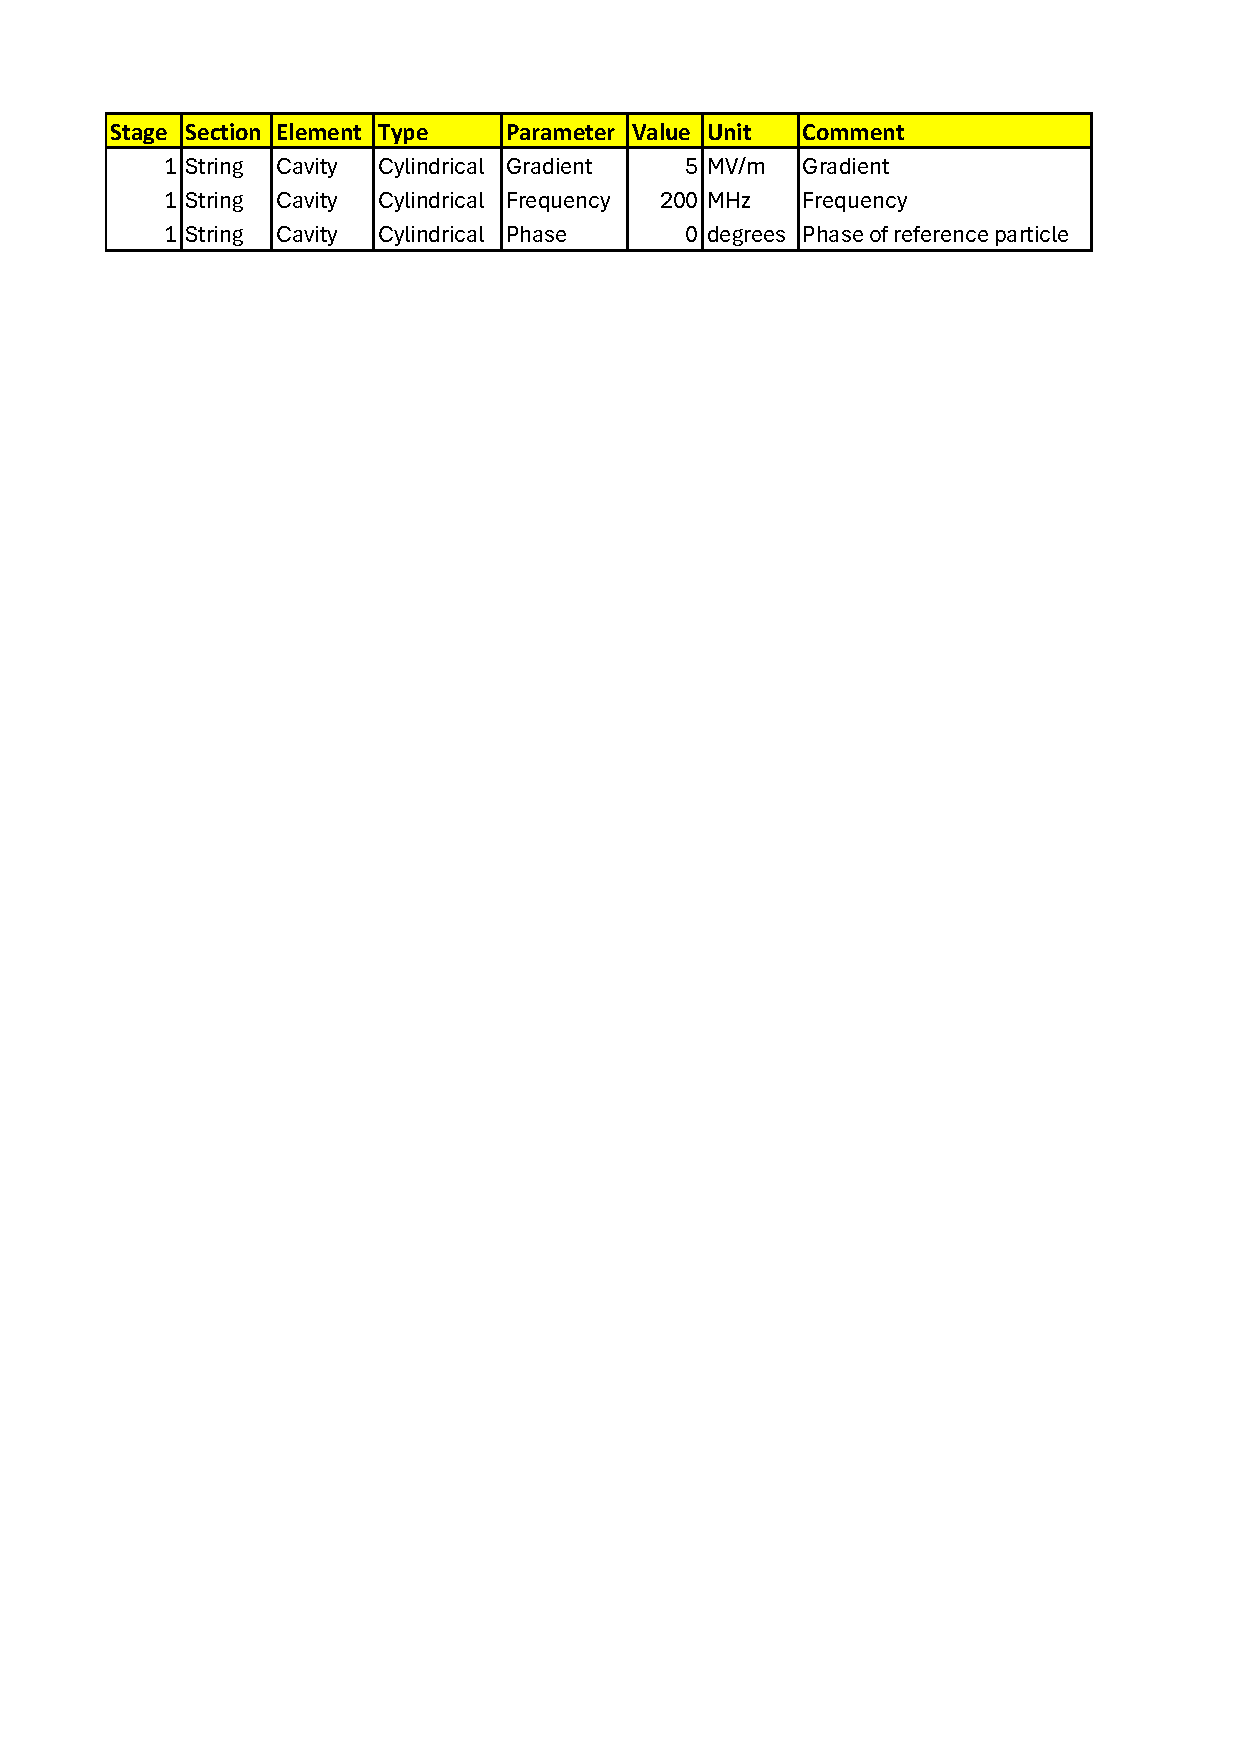
\includegraphics[width=0.95\textwidth]{CylindricalCavity.pdf}
  \end{center}
\end{table}

\paragraph{Instance attributes and access methods} ~\newline
\label{SubSubSect:CylndclRFCvty:InstAttr}
\noindent
The instance attributes are defined in
table~\ref{Tab:CylndclRFCvty:Attributes}. 
The attributes are accessed and set using the methods defined in
table~\ref{Tab:CylndclRFCvty:Methods}.
\begin{table}[h]
  \caption{
    Definition of attributes of instances of
    the \texttt{CylindricalRFCavity(BeamLineElement)} derived class.
    All attributes are required in the call to instantiate the
    element.
  }
  \label{Tab:CylndclRFCvty:Attributes}
  \begin{center}
    \begin{tabular}{|l|c|c|p{10cm}|}
      \hline
      \textbf{Attribute}   & \textbf{Type} & \textbf{Unit} & \textbf{Comment}                    \\
      \hline
      \texttt{Gradient}          & float & MV/m  & Peak electric field gradient on axis.         \\
      \texttt{Frequency}         & float & MHz   & Resonant frequency.                           \\
      \texttt{Phase}             & float & rad   & Phase cavity at time reference particle crosses
                                                   centre of cavity, ``linac convention''.       \\
      \texttt{TransitTimeFactor} & float &       & Transit time factor (equation~\ref{Eq:TrnsMat:CylCav:TransitTimeFactor}).  \\
      \texttt{V0}                & float & MV    & Peak voltage.                                 \\
      \texttt{alpha}             & float &       & $\alpha_{\rm RF}$ parameter defined in equation~\ref{Eq:TrnsMat:CylCav:alphaRF}. \\
      \texttt{wperp}             & float &       & $\omega_\perp$ parameter defined in equation~\ref{Eq:TrnsMat:CylCav:omegaPerp}. \\
      \texttt{cperp}             & float &       & $c_\perp$ parameter defined in equation~\ref{Eq:TrnsMat:CylCav:cPerp}. \\
      \texttt{sperp}             & float &       & $s_\perp$ parameter defined in equation~\ref{Eq:TrnsMat:CylCav:sPerp}. \\
      \texttt{wprll}             & float &       & $\omega_{||}$ parameter defined in equation~\ref{Eq:TrnsMat:CylCav:omegaParallel}. \\
      \texttt{cprll}             & float &       & $c_{||}$ parameter defined in equation~\ref{Eq:TrnsMat:CylCav:cParallel}. \\
      \texttt{sprll}             & float &       & $s_{||}$ parameter defined in equation~\ref{Eq:TrnsMat:CylCav:sParallel}. \\
      \hline
    \end{tabular}
  \end{center}
\end{table}
\begin{table}[h]
  \caption{
    Definition of access methods for the \texttt{CylindricalRFCavity} derived
    class. 
  }
  \label{Tab:CylndclRFCvty:Methods}
  \begin{center}
    \begin{tabular}{|c|c|p{5cm}|}
      \hline
      \textbf{Set method} & \textbf{Get method}  & \textbf{Comment}                                                 \\
      \hline
      \texttt{setGradient(Gradient)}        & \texttt{getGradient()}         & Set/get peak electric field gradient.      \\
      \texttt{setFrequency(Frequency)}      & \texttt{getFrequency()}        & Set/get frequency.       \\
      \texttt{setAngularFrequency(AngFreq)} & \texttt{getAngularFrequency()} & Set/get angular frequency. \\
      \texttt{setPhase(Phase)}              & \texttt{getPhase()}            & Set/get phase. \\ 
      \texttt{setWaveNumber(WaveNumber)}    & \texttt{getWaveNumber()}       & Set/get wavenumber.                     \\
      \texttt{setLength(Length)}            & \texttt{getLength()}           & Set/get Length. \\
      \texttt{setRadius(Radius)}            & \texttt{getRadius()}           & Set/get Radius. \\
      \texttt{setTransitTimeFactor}         & \texttt{getTransitTimeFactor()} & Set/get TransitTimeFactor. \\
      \quad\quad\quad \texttt{(TransitTimeFactor)} & & \\
      \texttt{setV0(V0)}                    & \texttt{getV0()}               & Set/get peak voltage.                     \\
      \texttt{setalpha(alpha)}              & \texttt{getalpha()}            & Set/get alpha.                     \\
      \texttt{setwperp(wperp)}              & \texttt{getwperp()}             & Set/get wperp.                     \\
      \texttt{setcperp(cperp)}              & \texttt{getcperp()}             & Set/get cperp.                     \\
      \texttt{setsperp(sperp)}              & \texttt{getsperp()}             & Set/get sperp.                     \\
      \texttt{setwprll(wprll)}              & \texttt{getwprll()}             & Set/get wprll.                     \\
      \texttt{setcprll(cprll)}              & \texttt{getcprll()}             & Set/get cprll.                     \\
      \texttt{setsprll(sprll)}              & \texttt{getsprll()}             & Set/get sprll.                     \\
      \texttt{setmrf(mrf)}                  & \texttt{getmrf()}              & Set/get mrf.                     \\
      \hline
    \end{tabular}
  \end{center}
\end{table}

\paragraph{Processing methods} ~\newline
\noindent
The \texttt{CylindricalRFCavity} derived class has no processing
methods other than those inheritted from the parent class.

\paragraph{I/o methods} ~\newline
\noindent
The \texttt{CylindricalRFCavity} derived class has no i/o methods other
than those inheritted from the parent class.

\paragraph{Utilities} ~\newline
\noindent
The \texttt{CylindricalRFCavity} derived class has no utilities other
than those inheritted from the parent class. 

\paragraph{Processing methods} ~\newline
\noindent
The \texttt{CylindricalRFCavity} dericed class has no processing methods.

\FloatBarrier

\subsubsection{Derived class: \texttt{Source(BeamLineElement)}}
\label{subsubSect:A1:BLE:Source}

\paragraph{Instantiation} ~\newline
\noindent
The call to instantiate the \texttt{Source} derived class is:
\begin{center}
  \texttt{Source(Name, rStrt, vStrt, drStrt, dvStrt,
          Mode, Parameters)}
\end{center}
Parent class arguments \texttt{Name}, \texttt{rStrt}, \texttt{vStrt},
\texttt{drStrt}, and \texttt{dvStrt} are described in
section~\ref{SubSubSect:BLE:InstAttr}.
These arguments are passed directly to \texttt{BeamLineElement}.
\texttt{Mode} is an integer that transmits the type of source to be
generated.
The specification of the \texttt{Parameters} list depends on the value
of \texttt{Mode}.
The content of the \texttt{Parameters} list is transferred directly to
the \texttt{Param} instance attribute.

The lines that specify the \texttt{Source} object in the beam-line
specification file are presented in table~\ref{App:MCD:Src:BS}. 
\begin{table}[h]
  \caption{
    Entries in the beam-line specification file that define the
    source object.
    \texttt{Stage} and \texttt{Section} may be speficied for
    convenience.
    These fields are used in creating the unique string that refers
    to the instance of the derived class.
    The groups of lines that define the source of each of the 
    four \texttt{Mode}s are indicated by the shading.
  }
  \label{App:MCD:Src:BS}
  \begin{center}
    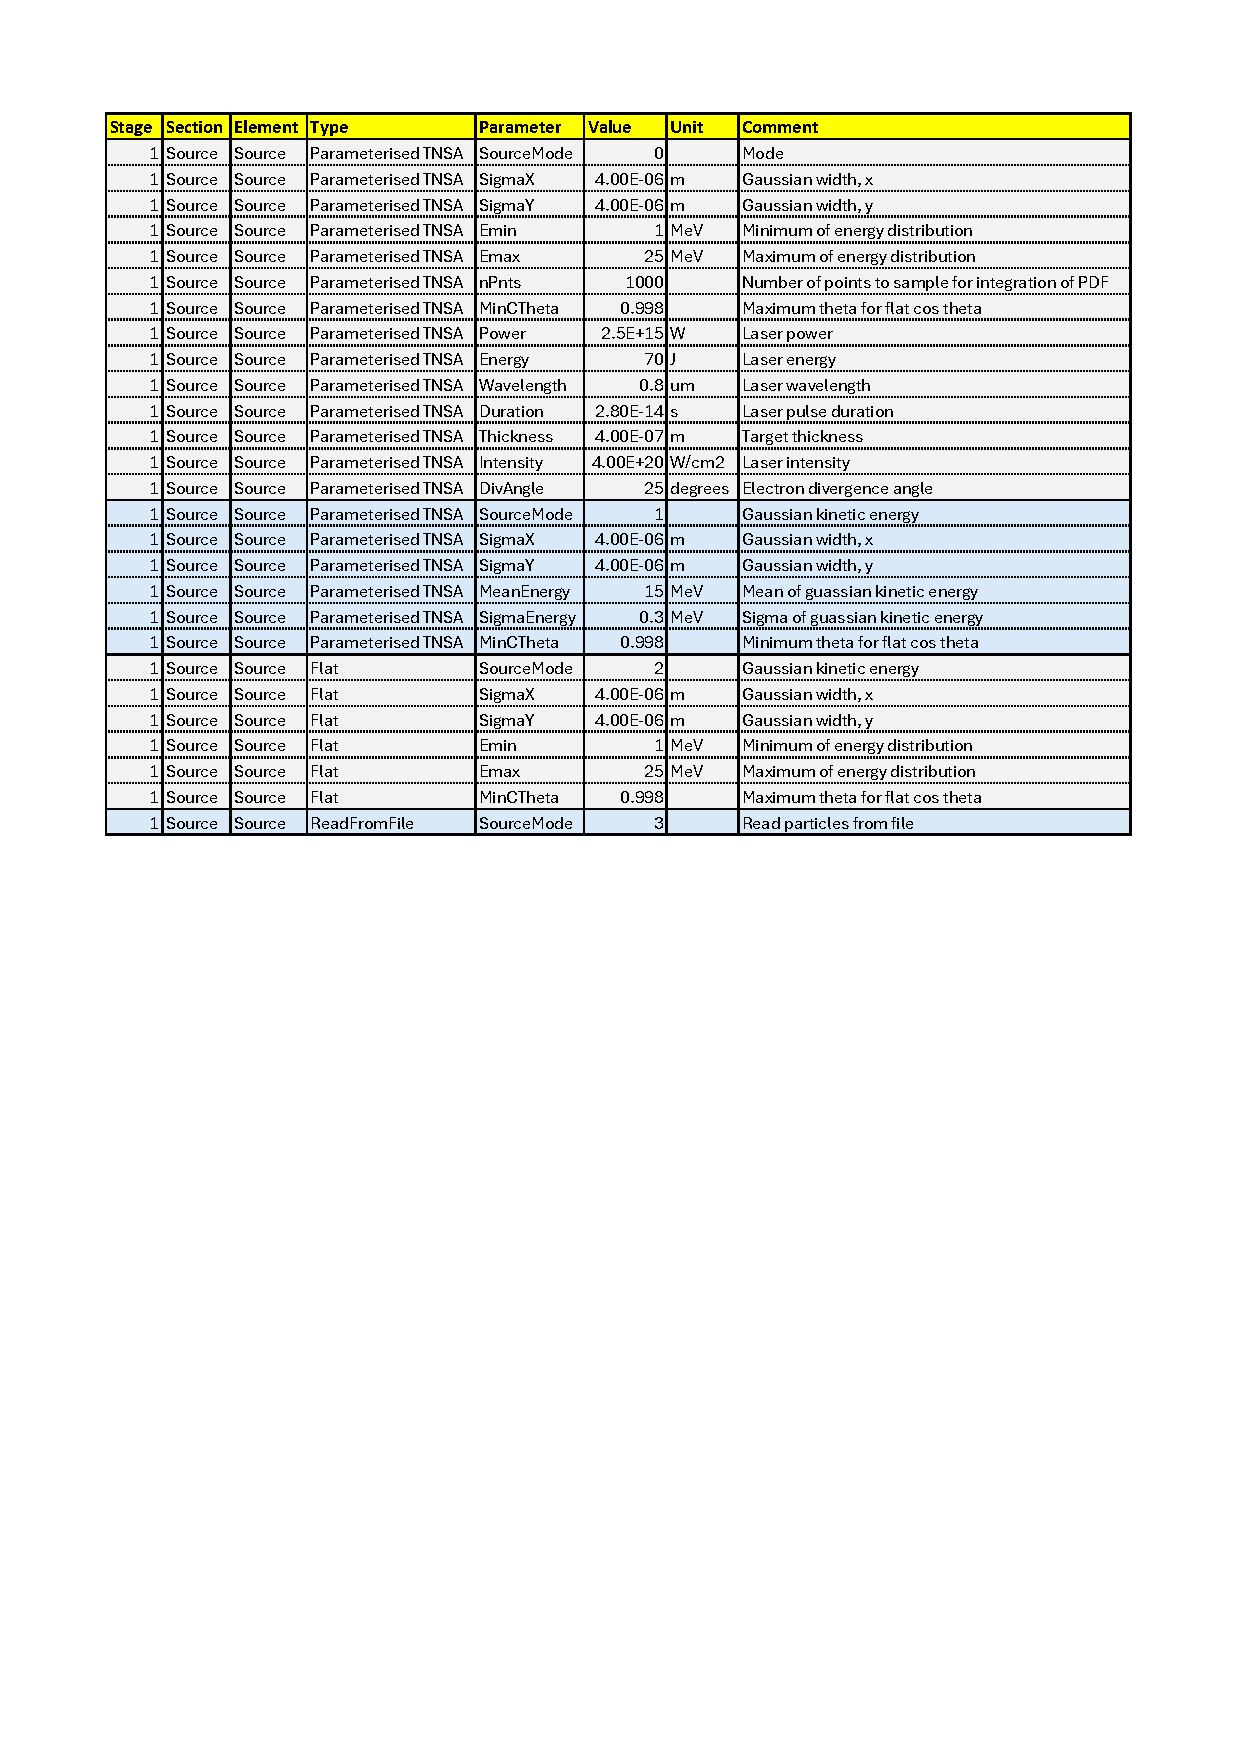
\includegraphics[width=0.95\textwidth]{Source.pdf}
  \end{center}
\end{table}

\paragraph{Instance attributes and access methods} ~\newline
\label{SubSubSect:Source:InstAttr}
\noindent
The instance attributes are defined in
tables~\ref{Tab:Source:AttributesA}, \ref{Tab:Source:AttributesB},
and \ref{Tab:Source:AttributesC}, each table refers to a particular
source \texttt{Mode}.
The attributes are accessed and set using the methods defined in
table~\ref{Tab:Source:Methods}.
\begin{table}[h]
  \caption{
    Definition of attributes of instances of
    the \texttt{Source(BeamLineElement)} derived class for
    source \texttt{Mode}$=0$, the parameterised TNSA model.
    All attributes are required in the call to instantiate the
    element.
  }
  \label{Tab:Source:AttributesA}
  \begin{center}
    \begin{tabular}{|l|c|c|p{10cm}|}
      \hline
      \texttt{Param[0]} & float   & $\mu$m   & $\lambda$: Laser wavelength.                                  \\
      \texttt{Param[1]} & float   & W        & $P_L$: Laser power.                                           \\
      \texttt{Param[2]} & float   & m        & $d$: Diameter of laser spot at focus.                        \\
      \texttt{Param[3]} & float   & s        & $t_{\rm laser}$: Laser pulse duration.                          \\
      \texttt{Param[4]} & float   & MeV      & Hot electron temperature.                                      \\
      \texttt{Param[5]} & float   & MeV      & Minimum kinetic energy ($K_{\rm min}$).                          \\
      \texttt{Param[6]} & float   & MeV      & Maximum kinetic energy ($K_{\rm max}$).                          \\
      \texttt{Param[7]} & float   & $^\circ$ & $\theta_{\rm degrees}$: Electron divergence angle.               \\
      \texttt{Param[8]} & float   & $^\circ$ & Intercept of $\alpha$, maximum half opening angle at $K=0$.    \\
      \texttt{Param[9]} & float   & $^\circ$ & Scaled slope of $\alpha(K)$.                                   \\
      \texttt{Param[10]} & float  &         & Maximum $\partial r / \partial s$. If given as -9999., then all values
                                              of $\partial r / \partial s$ are accepted.                               \\
      \hline
    \end{tabular}
  \end{center}
\end{table}
\begin{table}[h]
  \caption{
    Definition of attributes of instances of
    the \texttt{Source(BeamLineElement)} derived class for
    source \texttt{Mode}$=1$ in which energy is sampled from a normal
    distribution.
    All attributes are required in the call to instantiate the
    element.
  }
  \label{Tab:Source:AttributesB}
  \begin{center}
    \begin{tabular}{|l|c|c|p{10cm}|}
      \hline
      \textbf{Attribute} & \textbf{Type}      & \textbf{Unit} & \textbf{Comment}                    \\
      \hline
      \texttt{Mode}      & integer &          & \texttt{Mode}$=1$; parameterised laser-driven source.        \\
      \hline
       \texttt{Param[0]} & float   & m        & Standard deviation of normal distribution from which $x$ coordinate is sampled. \\
       \texttt{Param[1]} & float   & m        & Standard deviation of normal distribution from which $y$ coordinate is sampled. \\
       \texttt{Param[2]} & float   &          & Minimum $\cos\theta_S$.
                                                The specification of a minimum for $\cos\theta_S$ improves the efficiency of
                                                generation as it may be used to restrice generation to the set of partices that
                                                will enter the downstream acceptane.                                            \\
       \texttt{Param[3]} & float   & MeV      & Mean kinetic energy.                                          \\
       \texttt{Param[4]} & float   & MeV      & Standard deviation of kinetic energy distribution.            \\
      \hline
    \end{tabular}
  \end{center}
\end{table}
\begin{table}[h]
  \caption{
    Definition of attributes of instances of
    the \texttt{Source(BeamLineElement)} derived class for
    source \texttt{Mode}$=2$ in which energy is sampled from a uniform
    distribution.
    All attributes are required in the call to instantiate the
    element.
  }
  \label{Tab:Source:AttributesC}
  \begin{center}
    \begin{tabular}{|l|c|c|p{10cm}|}
      \hline
      \textbf{Attribute} & \textbf{Type}      & \textbf{Unit} & \textbf{Comment}                    \\
      \hline
      \texttt{Mode}      & integer &          & \texttt{Mode}$=2$; parameterised laser-driven source.        \\
      \hline
       \texttt{Param[0]} & float   & m        & Standard deviation of normal distribution from which $x$ coordinate is sampled. \\
       \texttt{Param[1]} & float   & m        & Standard deviation of normal distribution from which $y$ coordinate is sampled. \\
       \texttt{Param[2]} & float   &          & Minimum $\cos\theta_S$.
                                                The specification of a minimum for $\cos\theta_S$ improves the efficiency of
                                                generation as it may be used to restrice generation to the set of partices that
                                                will enter the downstream acceptane.                                            \\
       \texttt{Param[3]} & float   & MeV      & Mean kinetic energy.                                          \\
       \texttt{Param[4]} & float   & MeV      & Maximum kinetic energy.            \\
      \hline
    \end{tabular}
  \end{center}
\end{table}
\begin{table}[h]
  \caption{
    Definition of attributes of instances of
    the \texttt{Source(BeamLineElement)} derived class for
    source \texttt{Mode}$=3$ in which parameters of particle at source
    are read from an input file.
    All attributes are required in the call to instantiate the
    element.
  }
  \label{Tab:Source:AttributesD}
  \begin{center}
    \begin{tabular}{|l|c|c|p{10cm}|}
      \hline
      \textbf{Attribute} & \textbf{Type}      & \textbf{Unit} & \textbf{Comment}                    \\
      \hline
      \texttt{Mode}      & integer &          & \texttt{Mode}$=3$; partice trace space read from file.
                                                In this case no additional paramters are required. \\
      \hline
    \end{tabular}
  \end{center}
\end{table}
\begin{table}[h]
  \caption{
    Definition of access methods for the \texttt{Source} derived
    class. 
  }
  \label{Tab:Source:Methods}
  \begin{center}
    \begin{tabular}{|c|c|p{5cm}|}
      \hline
      \textbf{Set method} & \textbf{Get method}  & \textbf{Comment}                                                 \\
      \hline
      \texttt{setMode}             & \texttt{getMode()}          & Set/get Mode.                \\
      \texttt{setModeText}         & \texttt{getModeText()}      & Set string with readable name for mode.  \\
      \texttt{setModeParamterText} & \texttt{getParameterText()} & Set/get list of strings with readable name for paramter. \\
      \texttt{setParameters}       & \texttt{getParameters()}    & Set/get parameters; list of paramters as defined above. \\ 
      \texttt{setParameterUnit}    & \texttt{getParameterUnit()} & Set/get list of strings containing parameter units.  \\
      \hline
    \end{tabular}
  \end{center}
\end{table}

\paragraph{Processing methods} ~\newline
\noindent
The \texttt{Source} derived class has no processing
methods other than those inheritted from the parent class.

\paragraph{I/o methods} ~\newline
\noindent
The \texttt{Source} derived class has no i/o methods other
than those inheritted from the parent class.

\paragraph{Processing methods} ~\newline
\noindent
The processing methods provided by the \texttt{Source} derived class
are listed in table \ref{Tab:Source:Proc}.
\begin{sidewaystable}[h]
  \caption{
    Definition of processing methods provided by the \texttt{Source}
    derived class. 
  }
  \label{Tab:Source:Proc}
  \begin{center}
    \begin{tabular}{|c|c|c|p{7cm}|}
      \hline
      \textbf{Method} & \textbf{Arguments} & \textbf{Return}  & \textbf{Comment}                                                 \\
      \hline
      \texttt{getParticleFromSource()}       &         & ndarray       & Get trace space for particle at source, returns np.array.         \\
      \texttt{getParticle()}                 &         & floats        & Called from \texttt{getParticleFromSource()}, returns parameters
                                                                         used to create trace space of particle at source.                 \\
      \texttt{getFlatThetaPhi()}             &         & floats        & Called from \texttt{getParticle()} if flat $\cos\theta_S$, flat
                                                                         $\phi_S$ distribution is requested.                               \\
      \texttt{getgofrp(rpmax, xp, yp)}       & floats  & float         & Returns $g(r^\prime)$ given input $r^\prime_{\rm max}$, $x^\prime$,
                                                                         and $y^\prime$.                                                    \\
      \texttt{g\_theta(Energy)}              & float   &               & Returns $\theta_S$ generated using a guassian distribution.
                                                                         Depricated.                                                       \\
      \texttt{angle\_gemerator(Energy)}      & float   &               & Returns $\theta_S$, $\phi_S$ using \texttt{g\_theta} and uniform
                                                                         distribution for $\phi_S$.  Depricated.                           \\
      \texttt{getGaussianThetaPhi(Energy)}   & float   &               & Returns $\cos\theta_S$ and $\phi_S$ using \texttt{angle\_generator}. \\
      \texttt{paramters(P, E, l, tl, d, I, t)}& floats &               & Returns derived parameters used to generate TNSA proton kinetic
                                                                         energy spectrum.                                                  \\
      \texttt{equation(x, tl, t0)}          & floats  &               & Returns result of evaluation equation~\ref{EquforX}.                   \\
      \texttt{getLaserDrivenProtonEnergy()} &         &               & Generates proton kinetic energy at source for paramterised TNSA
                                                                         model.                                                            \\
      \texttt{getLaserCumProbParam()} &         &               &                                                             \\
      \texttt{getLaserCumProb()} &         &               &                                                             \\
      \texttt{getLaserDrivenProtonEnergyProbDensity()} &         &               &                                                             \\
      \texttt{getTraceSpace()} &         &               &                                                             \\
      \hline
    \end{tabular}
  \end{center}
\end{sidewaystable}

\paragraph{Utilities} ~\newline
\noindent
The utilities provided by the \texttt{Source} derived class are listed
in table \ref{Tab:Source:Utils}.
\begin{table}[h]
  \caption{
    Definition of utilities provided by the \texttt{Source}
    derived class. 
  }
  \label{Tab:Source:Utils}
  \begin{center}
    \begin{tabular}{|c|c|c|p{5cm}|}
      \hline
      \textbf{Method} & \textbf{Arguments} & \textbf{Return}  & \textbf{Comment}                                                 \\
      \hline
      \texttt{CheckSourceParam(Mode, Param)} & Integer, list & boolean & Class method. Check that mode and parameters are valid.
                                                                         Calls \texttt{CheckMode} and \texttt{CheckParam}                  \\
      \texttt{CheckMode(Mode)}               & integer & boolean       & Class method. Check is valid.                                     \\
      \texttt{CheckParam}                    & list    & boolean       & Class method. Check paramter list is valid.                       \\
      \texttt{tabulateParameters()} &         &               &                                                             \\
      \hline
    \end{tabular}
  \end{center}
\end{table}

\subsection{\texttt{UserFramework}}
\label{SubSubSect:UsrFrmwrk}

\texttt{UserFramework} is a module that provides a set of methods used
in the code provided to allow users easy access to the code and data.
The following methods are provided: \\
\begin{description}
  \item{\texttt{startAnalysis(argv)}}: processes input flags passed
    in call to run script.  \\
    Argument:
    \begin{description}
      \item{\texttt{argv}}: list of arguments passed to \texttt{main}
        by call to run script.
    \end{description}
    Returns:
    \begin{description}
      \item{\texttt{Success}}:      (boolean) True if processing successful.
      \item{\texttt{Debug}}:        (boolean) Set to True if
                                    flag \texttt{-d} is set to True.
      \item{\texttt{inputfile}}:    (path) full path to input file; set
                                    using flag \texttt{-y}.
      \item{\texttt{outputfile}}:   (path) full path to output file; set
                                    using flag \texttt{-o}.
      \item{\texttt{nEvts}}:        (integer) number of events to
                                    process; set using flag \texttt{-n}.
      \item{\texttt{bdsimfile}}:    (path) full path to bdsim format file; set
                                    using flag \texttt{-z}.
      \item{\texttt{beamspecfile}}: (path) full path to beam
                                    specification CSV file; set
                                    using flag \texttt{-b}. \\
    \end{description}
    
  \item{\texttt{handleFILES(beamspecfile, inputfile, outputfile, bdsimFILE=False)}}: 
    File handling method to check files exist and create
    relevant \texttt{BeamIO} instances. \\
    Arguments:
    \begin{description}
      \item{\texttt{beamspecfile}}: (path) full path to beam
                                    specification CSV file;
      \item{\texttt{inputfile}}:    (path) full path to input file;
      \item{\texttt{outputfile}}:   (path) full path to output file;
      \item{\texttt{bdsimfile}}:    (path) full path to bdsim format file.
    \end{description}
    Returns:
    \begin{description}
      \item{\texttt{Success}}: (boolean) True if file handling successful.
      \item{\texttt{ibmIOr}}:  (\texttt{BeamIO}) instance
                               of \texttt{BeamIO} class for file to be read.
      \item{\texttt{ibmIOw}}:  (\texttt{BeamIO}) instance
                               of \texttt{BeamIO} class for file to be
                               written. \\
    \end{description}
    
  \item{\texttt{EventLoop(iUsrAnl, ibmIOr, ibmIOw, nEvtsIn)}}:
    executes loop over \texttt{nEvtsIn} events.
    Reads event record or generates event if \texttt{ibmIOr}$=$None,
    and handles end-of-file.
    Passes control to \texttt{UserAnal.EventLoop}.   \\
    Arguments:
    \begin{description}
      \item{\texttt{iUsrAnl}}: (\texttt{UserAnal}) instance.
      \item{\texttt{ibmIOr}}:  (\texttt{BeamIO}) instance
                               of \texttt{BeamIO} class for file to be read.
      \item{\texttt{ibmIOw}}:  (\texttt{BeamIO}) instance
                               of \texttt{BeamIO} class for file to be
                               written.
      \item{\texttt{nEvtsIn}}: (integer) number of events to
                               process.
    \end{description}
    Returns:
    \begin{description}
      \item{\texttt{Success}}: (boolean) True if successful.
    \end{description}
\end{description}

\subsection{\texttt{visualise}}
\label{SubSect:vis}

The \texttt{visualise} class manages the visualisation of the beam
line and particles traversing it.

\subsubsection{Instantiation}
\noindent
The call to instantiate the \texttt{visualise} class is:
\begin{center}
  \texttt{Beam(CoordSys, Projection)}
\end{center}
\texttt{CoordSys} (string) is either ``RPLC'' to visualise the beam
line in the reference particle local coordinate system or ``Lab''.
\texttt{Projection} (string) is either ``$xs$'' (RPLC) or ``$xz$''
(lab) to visualise the $xs$ or $xz$ projecton and eithed ``$ys$''
(RPLC) or ``$yz$'' (lab) to visualise the $xs$ or $xz$ projecton.

\subsubsection{Instance attributes and access methods}
\label{Para:vis:InstAttr}
\noindent
The instance attributes are presented in table~\ref{Tab:vis:Attributes}
and the access methods are summarised in table~\ref{Tab:vis:AccessMethods}.
\begin{table}[h]
  \caption{
    Definition of attributes of instances of the \texttt{visualise} class.
  }
  \label{Tab:vis:Attributes}
  \begin{center}
    \begin{tabular}{|l|c|p{12cm}|}
      \hline
      \textbf{Attribute} & \textbf{Type} & \textbf{Comment}                \\
      \hline
      \texttt{CoordSys}  & String & Either ``RPLC'' to visualise the
                                    in the reference particle local
                                    coordinate system or ``Lab''.         \\
      \texttt{Projection}& String & Either ``$xs$'' (RPLC) or ``$xz$''
                                    (lab) to visualise the $xs$ or
                                    $xz$ projecton and eithed ``$ys$'' 
                                    (RPLC) or ``$yz$'' (lab) to
                                    visualise the $xs$ or $xz$
                                    projecton.                            \\
       \hline
    \end{tabular}
  \end{center}
\end{table}
\begin{table}[h]
  \caption{
    Definition of access methods for the \texttt{visualise}
    class. 
  }
  \label{Tab:vis:AccessMethods}
  \begin{center}
    \begin{tabular}{|c|c|p{11cm}|}
      \hline
      \textbf{Set method} & \textbf{Get method}  & \textbf{Comment}                                  \\
      \hline
      \texttt{setCoordSys}     & \texttt{getCoordSys}   & Set coordinate system for visualisation.     \\
      \texttt{setProjection}   & \texttt{setProjection} & Set projection for visualisation.            \\
      \hline
    \end{tabular}
  \end{center}
\end{table}

\subsubsection{Processing methods}
\noindent
Table~\ref{Tab:vis:ProcMethods} presents the processing methods provided
in the \texttt{visualise} class.
\begin{table}[h]
  \caption{
    Processing methods provided by the \texttt{visualise}
    class. 
  }
  \label{Tab:vis:ProcMethods}
  \begin{center}
    \begin{tabular}{|l|c|c|p{7cm}|}
      \hline
      \textbf{Method} & \textbf{Argument(s)} & \textbf{Return} & \textbf{Comment}                                                       \\
      \hline
      \texttt{Particles(axs, nPrtcl)} & plot, integer  & & Manage ploting of \texttt{nPrtcl} particles on \texttt{matplotlib} \texttt{axes}
                                                           instance.                                                                    \\
      \texttt{BeamLine(axs)}          & plot           & & Manage ploting of beam line on \texttt{matplotlib} \texttt{axes} instance.   \\
      \hline
    \end{tabular}
  \end{center}
\end{table}

\subsubsection{I/o methods}
\noindent
The \texttt{visualise} class has no i/o methods.

\subsubsection{Utilities}
\noindent
The \texttt{visualise} class has no i/o methods.

\FloatBarrier

\subsection{\texttt{BeamIO}}
\label{SubSect:BmIO}

The \texttt{BeamIO} class provides interfaces to the reading and
writing of beam specification and beam data files.

\subsubsection{Instantiation}
\noindent
The call to instantiate the \texttt{BeamIO} class is:
\begin{center}
  \texttt{BeamIO(datafilePATH, datafileNAME, create, BDSIMfile)}
\end{center}
\begin{description}
  \item{\texttt{datafilePATH}}: (string) Path to directory in which
    input file is to be found, or, in which output file is to be
    created. 
    \texttt{datafilePATH} can be set to  None if the full path is
    specified in \texttt{datafileNAME}.
  \item{\texttt{datafileNAME}}: (string) File name (string) which,
    when appendded to \texttt{datafilePATH} gives the full path to the
    input or output data file, or. full path to the input or output
    file.
  \item{\texttt{create}}: (boolean) if true indicates that the file
    must be created.
    If a file exists at the location specified
    by \texttt{datafilePATH} and \texttt{datafileNAME} it will be
    overwritten.
  \item{\texttt{BDSIMfile}}: (boolean) If True then the file is to be
    read or written in \texttt{BDSIMfile} format.
\end{description}

\subsubsection{Instance attributes and access methods}
\label{Para:BmIO:InstAttr}
\noindent
The \texttt{BeamIO} instance attributes are presented in
table~\ref{Tab:BmIO:Attributes} and the access methods are summarised
in table~\ref{Tab:BmIO:AccessMethods}.
\begin{table}[h]
  \caption{
    Definition of attributes of instances of the \texttt{BeamIO} class.
  }
  \label{Tab:BmIO:Attributes}
  \begin{center}
    \begin{tabular}{|l|c|p{11cm}|}
      \hline
      \textbf{Attribute} & \textbf{Type} & \textbf{Comment}                \\
      \hline
      \texttt{dataFILE}        & Path    & Full path to data file.                  \\
      \texttt{Read1stRecord}   & Boolean & True if first record has been read from file. \\
      \texttt{dataFILEversion} & Integer & For \texttt{BeamIO} files version number identifying file format. \\
      \texttt{create}          & Boolean & True if data file is to be created. \\
      \texttt{BDSIMfile}       & Boolean & True id reading or writing a BDSim file. \\
       \hline
    \end{tabular}
  \end{center}
\end{table}
\begin{table}[h]
  \caption{
    Definition of access methods for the \texttt{BeamIO}
    class. 
  }
  \label{Tab:BmIO:AccessMethods}
  \begin{center}
    \begin{tabular}{|c|c|p{7.5cm}|}
      \hline
      \textbf{Set method} & \textbf{Get method}  & \textbf{Comment}                                                                 \\
      \hline
      \texttt{setpathFILE}        & \texttt{getpathFILE}        & Set/get path to directory containing data file.                   \\
      \texttt{setdataFILE}        & \texttt{getdataFILE}        & Set/get full path to data file.                                   \\
      \texttt{setReadFirstRecord} & \texttt{getReadFirstRecord} & Set/get flag indicating whether the first record has been read.   \\
      \texttt{setcreate}          & \texttt{getcreate}          & Set/get flag indicating whether data file is to be created.       \\
      \texttt{setdataFILEversion} & \texttt{getdataFILEversion} & Set/get \texttt{BeamIO} version number.                           \\
      \texttt{setBDSIMfile}       & \texttt{getBDSIMfile}       & Set/get flag indicating whether the data file is in BDSIM format. \\
      \hline
    \end{tabular}
  \end{center}
\end{table}

\subsubsection{Processing methods}
\noindent
The \texttt{BeamIO} class has no processing methods.

\subsubsection{I/o methods}
\noindent
Table~\ref{Tab:BmIO:IoMethods} presents the i/o methods provided by the
\texttt{BeamIO} class.
\begin{table}[h]
  \caption{
    I/o methods provided by the \texttt{BeamIO} class. 
  }
  \label{Tab:BmIO:IoMethods}
  \begin{center}
    \begin{tabular}{|l|c|c|p{5cm}|}
      \hline
      \textbf{Method} & \textbf{Argument(s)} & \textbf{Return} & \textbf{Comment}                                        \\
      \hline
      \texttt{readBeamDataRecord()}  &   & Boolean & Manages reading/writing of a record from/to the data file.
                                           Returns a boolean, \texttt{EoF}, set to True of end of file has been detected. \\
      \texttt{writeFIRSTword()}      &   &         & Writes \texttt{9999} to indicate that \texttt{BeamIO} version is $>1$.
                                           Returns integer version number.                                                \\
      \texttt{writeVersion(version)} & string &    & Writes data-file format version to file.  Version is a string, e.g.
                                                       \texttt{BeamIO V3}.                                                \\
      \texttt{readVersion()}         &   & Integer & Reads data-file format version number from file.
                                           Returns integer version number stripped from end of string (e.g. 3).           \\
      \texttt{writeREPOversion()}    &   &         & Writes git repo Tag label, together with date/time and text description
                                                     of last commit, together with date/time.                             \\
      \texttt{readREPOversion()}     &   & list    & Reads and returns list of strings containing git repo Tag label,
                                                     together with date/time and text description of last commit, together
                                                     with date/time.                                                      \\
      \texttt{flushNclosedataFile(dataFILE)} & Path &     & Flush and close data \texttt{dataFILE} at end of processing.  \\
      \hline
    \end{tabular}
  \end{center}
\end{table}

\subsubsection{Utilities}
\noindent
Table~\ref{Tab:BmIO:Utils} presents the utilities provided by the
\texttt{BeamIO} class.
\begin{table}[h]
  \caption{
    Utilities provided by the \texttt{BeamIO} class. 
  }
  \label{Tab:BmIO:Utils}
  \begin{center}
    \begin{tabular}{|l|c|c|p{7cm}|}
      \hline
      \textbf{Method} & \textbf{Argument(s)} & \textbf{Return} & \textbf{Comment}                                     \\
      \hline
      \texttt{resetinstances()}   &  &  & Class method. Sets list of instances to \texttt{[]}.                        \\
      \texttt{cleanBeamIOfiles()} &  &  & Class method. Delete \texttt{BeamIO} instances and reset list of instances. \\
      \hline
    \end{tabular}
  \end{center}
\end{table}

\subsection{\texttt{Simulation}}
\label{SubSect:Simu}

The singleton \texttt{Simulation} class provides a framework and
utilities for the simulation of the passage of particles through the
beam lines defined through the classes described in this document.
By default the seed for the random number generator is set using the
system time.

\subsubsection{Instantiation}
\noindent
The call to instantiate the \texttt{Simulation} class is:
\begin{center}
  \texttt{Simulation(NEvts, BeamLineSpecificationCVSfile, dataFileDir, dataFileName)}
\end{center}
\begin{description}
  \item{\texttt{NEvts}}: (integer) Number of events to generate.
  \item{\texttt{BeamLineSpecificationCVSfile}}: (string) String
    containing path to the beam-line specification CVS file.
  \item{\texttt{dataFileDir}}: (string) String containing path
    to directory in which data file is to be written.
  \item{\texttt{dataFileName}}: (string) Name of file to be written.
\end{description}

\texttt{Simulation} has two methods defined outside the class:
\begin{description}
  \item{\texttt{getRandom()}}: returns number between $0.$ and $1.$
    drawn from a uniform distributin; and 
  \item{\texttt{getParabolic(umax)}}: returns number between
    $-\texttt{umax}$ and $\texttt{umax}$ drawn from a parabolic
      distribution with a maximum at 0. 
\end{description}
\subsubsection{Instance attributes and access methods}
\label{Para:Simu:InstAttr}
\noindent
The \texttt{Simulation} instance attributes are presented in
table~\ref{Tab:Simu:Attributes} and the access methods are summarised
in table~\ref{Tab:Simu:AccessMethods}.
\begin{table}[h]
  \caption{
    Definition of attributes of instances of the \texttt{Simulation} class.
  }
  \label{Tab:Simu:Attributes}
  \begin{center}
    \begin{tabular}{|l|c|p{11cm}|}
      \hline
      \textbf{Attribute} & \textbf{Type} & \textbf{Comment}                                                                      \\
      \hline
      \texttt{NEvt}          & integer  & Number of events to generate.                                                          \\
      \texttt{ParamFileName} & string   & Path to beam-line parameter CSV file.                                                  \\
      \texttt{dataFileDir}   & string   & Path to the directory in which data file is to be written.                             \\
      \texttt{dataFileName}  & string   & Name of file to be created.                                                            \\
      \texttt{Facility}      & Facility & Instance of the derived \texttt{Facility} class derived from \texttt{BeamLineElement}. \\
      \texttt{iBmIOw}        & BeamIO   & Instance of the derived \texttt{BeamIO} class for the file to be written.              \\
      \texttt{ProgressPrint} & boolean  & If True the progress towards the \texttt{NEvt} requested events is printed.            \\
      \hline
    \end{tabular}
  \end{center}
\end{table}
\begin{sidewaystable}[h]
  \caption{
    Definition of access methods for the \texttt{Simulation}
    class. 
  }
  \label{Tab:Simu:AccessMethods}
  \begin{center}
    \begin{tabular}{|c|c|p{9.5cm}|}
      \hline
      \textbf{Set method} & \textbf{Get method}  & \textbf{Comment}                                                                                       \\
      \hline
      \texttt{setNEvt}                      & \texttt{getNEvt}                      & Set/get number of events to generate.                               \\
      \texttt{setBeamLineSpecificationFile} & \texttt{getBeamLineSpecificationFile} & Set/get full path to beam line specification file.                  \\
      \texttt{setdataFileDir}               & \texttt{getdataFileDir}               & Set/get path to directory in which data file is to be written.      \\
      \texttt{setdataFileName}              & \texttt{getdataFileName}              & Set/get name of data file to be created.                            \\
      \texttt{setFacility}                  & \texttt{getFacility}                  & Set/get \texttt{Facility} instance.                                 \\
      \texttt{setiBmIOw}                    & \texttt{getiBmIOw}                    & Set/get \texttt{BeamIO} instance specifying the file to be written. \\
      \texttt{setProgressPrint}             & \texttt{getProgressPrint}             & Set/get flag that controls the progress printout.                   \\
      \hline
    \end{tabular}
  \end{center}
\end{sidewaystable}

\subsubsection{Processing methods}
\noindent
The \texttt{Simulation} class provides one processing method:
\begin{center}
  \texttt{RunSim()}
\end{center}
which manages the generation of \texttt{NEvts} events.
The specification of the beam line and the individual events are
written to the output data file.

\subsubsection{I/o methods}
\noindent
The \texttt{Simulation} class provides no i/o methods.

\subsubsection{Utilities}
\noindent
The \texttt{Simulation} provides no utilities.

\subsection{\texttt{Physical constants}}
\label{SubSect:PhysCnsts}

The \texttt{PhysicalConstants} class provides the physical constants
that are required to carry out the linear optics calculations. 
The values are taken from, for example, the Particle Data Group book.
The constants packages is implemented as a singleton class so that
there is no ambiguity about which values are in use. 

\subsubsection{Instantiation}
\noindent
The call to instantiate the \texttt{PhysicalConstants} class is:
\begin{center}
  \texttt{PhysicalConstants()}
\end{center}

\subsubsection{Instance attributes and access methods}
\label{Para:PhysCnsts:InstAttr}
\noindent
The \texttt{PhysicalConstants} has no instance attributes.
The access methods are summarised in
table~\ref{Tab:PhysCnsts:AccessMethods}.
\begin{table}[h]
  \caption{
    Definition of access methods for the \texttt{PhysicalConstants}
    class. 
  }
  \label{Tab:PhysCnsts:AccessMethods}
  \begin{center}
    \begin{tabular}{|c|c|p{7cm}|}
      \hline
      \textbf{Set method} & \textbf{Get method}  & \textbf{Comment}                                                                                       \\
      \hline
        & \texttt{getPDGref}   & Returns PDG reference used.                               \\
        & \texttt{getSoL} & Returns speed of light in m/s.                  \\
        & \texttt{getSpecies}      & Returns list of particle species for which constants are stored. \\
        & \texttt{getParticleMASS(Species)}  & Returns particle mass for \texttt{Species}.
                                               Species is a list of strings:
                                               \texttt{["proton", "pion", "muon", "neutrino"]}. \\
        & \texttt{mp}                        & Returns proton mass in MeV. \\
        & \texttt{getmPion}                  & Returns pion mass in MeV. \\
        & \texttt{getmMuon}                  & Returns muon mass in MeV. \\
        & \texttt{getmNeutrino}              & Returns 0, neutrino mass (for \texttt{nuSIM}). \\
        & \texttt{getm0}                     & Returns permittivity of free space.                   \\
      \hline
    \end{tabular}
  \end{center}
\end{table}

\subsubsection{Processing methods}
\noindent
The \texttt{PhysicalConstants} class provides no processing methods.

\subsubsection{I/o methods}
\noindent
The \texttt{PhysicalConstants} class provides no i/o methods.

\subsubsection{Utilities}
\noindent
The \texttt{PhysicalConstants} provides no utilities.

\FloatBarrier

\subsection{\texttt{Report}}
\label{SubSect:Rprt}

The \texttt{Report} parent class supports a collection of derived
classes to generate reports, usually in the form of a CSV file, based
on the data stored in the attributes of
the \texttt{Beam}, \texttt{BeamLine}, \texttt{BeamLineElement}, \texttt{Particle},
and other classes.

\subsubsection{Instantiation}
\noindent
The call to instantiate the \texttt{Report} class is:
\begin{center}
  \texttt{Report(Name, ReportPath, FileName, Header, Lines)}
\end{center}
\begin{description}
  \item{\texttt{Name}}: (string) Name of report;
  \item{\texttt{ReportPath}}: (string) String containing path to the
    directory where report will be written; 
  \item{\texttt{FileName}}: (string) String containing name of the
   file in which report will be written.
  \item{\texttt{Header}}: (list of strings) List containing strings
    that will form the header record of the report; and
  \item{\texttt{Lines}}: (list of lists) The lines that will
    make up the lines of the report.
    List[i][j] provides the value of the item to be recorded in
    column \texttt{j} of row \texttt{i} of the report.
\end{description}

\subsubsection{Instance attributes and access methods}
\label{Para:Rprt:InstAttr}
\noindent
The \texttt{Report} parent class supports a collection of derived
classes to generate reports, usually in the form of a CSV file, based
on the data stored in the attributes of
the \texttt{Beam}, \texttt{BeamLine}, \texttt{BeamLineElement}, \texttt{Particle},
and other classes.
instance attributes are presented in
table~\ref{Tab:Rprt:Attributes} and the access methods are summarised
in table~\ref{Tab:Rprt:AccessMethods}.
\begin{table}[h]
  \caption{
    Definition of attributes of instances of the \texttt{Report} class.
  }
  \label{Tab:Rprt:Attributes}
  \begin{center}
    \begin{tabular}{|l|c|p{11cm}|}
      \hline
      \textbf{Attribute} & \textbf{Type} & \textbf{Comment}                                                                      \\
      \hline
      \texttt{NEvt}          & integer  & Number of events to generate.                                                          \\
      \texttt{ParamFileName} & string   & Path to beam-line parameter CSV file.                                                  \\
      \texttt{dataFileDir}   & string   & Path to the directory in which data file is to be written.                             \\
      \texttt{dataFileName}  & string   & Name of file to be created.                                                            \\
      \texttt{Facility}      & Facility & Instance of the derived \texttt{Facility} class derived from \texttt{BeamLineElement}. \\
      \texttt{iBmIOw}        & BeamIO   & Instance of the derived \texttt{BeamIO} class for the file to be written.              \\
      \texttt{ProgressPrint} & boolean  & If True the progress towards the \texttt{NEvt} requested events is printed.            \\
      \hline
    \end{tabular}
  \end{center}
\end{table}
\begin{table}[h]
  \caption{
    Definition of access methods for the \texttt{Report}
    class. 
  }
  \label{Tab:Rprt:AccessMethods}
  \begin{center}
    \begin{tabular}{|c|c|p{9.5cm}|}
      \hline
      \textbf{Set method} & \textbf{Get method}  & \textbf{Comment}                                                       \\
      \hline
      \texttt{setName}       & \texttt{getName}       & Set/get name of report.                                           \\
      \texttt{setReportPath} & \texttt{getReportPath} & Set/get path to director into which report file is to be written. \\
      \texttt{setFileName}   & \texttt{getFileName}   & Set/get name of file to be written.                               \\
      \texttt{setHeader}     & \texttt{getHeader}     & Set/get list of strings forming header fields.                    \\
      \texttt{setLines}      & \texttt{getLines}      & Set/get list of lists containing report entries line by line.     \\
      \hline
    \end{tabular}
  \end{center}
\end{table}

\subsubsection{Processing methods}
\noindent
Table~\ref{Tab:Rprt:ProcMethods} presents the processing methods provided
in the \texttt{Report} class.
\begin{table}[h]
  \caption{
    Processing methods provided by the \texttt{Report}
    class. 
  }
  \label{Tab:Rprt:ProcMethods}
  \begin{center}
    \begin{tabular}{|l|c|c|p{5cm}|}
      \hline
      \textbf{Method} & \textbf{Argument(s)} & \textbf{Return} & \textbf{Comment}                                                       \\
      \hline
      \texttt{createPandasDataFrame()} & & Data frame instance & Create pandas data frame using the data contained in \texttt{Header}
                                                                 and \texttt{Lines}.
                                                                 The instance is returned.                                              \\
      \hline
    \end{tabular}
  \end{center}
\end{table}

\subsubsection{I/o methods}
\noindent
Table~\ref{Tab:Rprt:IoMethods} presents the i/o methods provided in
the \texttt{Report} class.
\begin{table}[h]
  \caption{
    I/o methods provided by the \texttt{Report} class. 
  }
  \label{Tab:Rprt:ProcMethods}
  \begin{center}
    \begin{tabular}{|l|c|c|p{7cm}|}
      \hline
      \textbf{Method} & \textbf{Argument(s)} & \textbf{Return} & \textbf{Comment}                                                       \\
      \hline
      \texttt{createCSV(DataFrame)} & Data frame instance & & Create CSV file from pandas data \texttt{DatsFrame} frame using the data
                                                              contained in \texttt{Header} and \texttt{Lines}.                          \\
      \texttt{asCSV()}              &                     & & Write pandas dataframe and write it to CSV file.                          \\
      \hline
    \end{tabular}
  \end{center}
\end{table}

\subsection{\texttt{LaTeX}}
\label{SubSect:LTX}

The \texttt{LaTeX} module provides 2 methods to support the generation
of LaTeX tables from data stored in the class and instance attributes.
The first method, \texttt{TableHeader}, creates the header of LaTeX
table.
The method is accessed via the call:
\begin{center}
  \texttt{TableHeader(FilePath, TabString, Caption)}
\end{center}
where:
\begin{description}
  \item{\texttt{FilePath}}: (path) is the full path to the file to
    contain the table;
  \item{\texttt{TabString}}: (string) is the string that defines the
    columns, e.g., \texttt{'|c|c|'}, would result in a two-column
    table in which the contents of each column is centred; and
  \item{\texttt{Caption}}: (string) Is the string to be used as the
    table caption; and
\end{description}
Each line in the table are entered with the call:
\begin{center}
  \texttt{TableLine(FilePath, Line)}
\end{center}
where:
\begin{description}
  \item{\texttt{FilePath}}: (path) is the full path to the file to
    contain the table;
  \item{\texttt{Line}}: (string) is a list of strings that contain the
    contents of the line.
    A typical use case would be to create the table header, enter a
    line containing the header fields and then procede to add each
    line in the table in turn; and
    LaTeX commants are allowed, e.g. \texttt{Line = $\backslash$hline}
    will produce a horizontal line.
\end{description}
The final lines of LaTeX code is entered with the call:
\begin{center}
  \texttt{TableTrailer(FilePath)}
\end{center}
where:
\begin{description}
  \item{\texttt{FilePath}}: (path) is the full path to the file to
    contain the table.
\end{description}

\FloatBarrier
